\chapter{Partitioned Priors}

One way in which we may try to improve the performance of local, single-site, Metropolis-Hastings is by paritioning the prior distribution into several component parts. The idea behind this approach is that we may be able to guide the resampling process as to improve the rate of convergence to the mode and the mixing properties of local Metropolis-Hastings. \todo{say something about proposal kernels vs. sampling from prior?} If this approach proves succesful, it would enable us to design a light pre-inference rewriting of a probabilistic program which splits up its priors so that the subsequent inference step is performed more efficiently.

In this chapter we focus on the splitting of uniform continuous priors. Not only are such priors commonly used in models, but sampling from any distribution ultimately relies on uniformly drawn random bits. Speeding up inference on uniform priors may therefore lead to speed ups on other distributions, assuming certain desirable properties, such that small changes in the uniform bits correspond to small changes in the final distribution. \todo{not sure if this makes much sense. Need to research it or remove}

For simplicity, we focus on models with a uni-modal posterior distribution. The analysis for multi-modal distributions would follow similar lines to the one presented here, but would also have to additionally account for mode-switching.

\section{Preliminaries}

In order to explore the partitioned prior idea we need to have an understanding of the basic Metropolis-Hastings algorithm. We also need a way to evaluate the performance of a certain partition, which we propose to do by looking separately at the time it takes for our Markov Chain to reach the true posterior's mode and at the chain's mixing properties around this mode.

\subsection{Metropolis-Hastings}
\label{sect:MH}
The Metropolis-Hastings algorithm is a method of drawing samples from a probability distribution $P(x)$ when we can only compute values of the proportional function $P^*(x) = P(x)*Z$. This method is usefull when we want to estimate distributions (or expectations under distributions) that we cannot directly evaluate, which is a common problem in Bayesian modelling, since the probability distribution's normalization factor is often difficult to estimate.

Metropolis-Hastings is a Markov Chain Monte Carlo algorithm, which is to say that the algorithm will generate samples according to the Markov, memoryless, property where the choice of current sample depends only on the previous sample. Additionally, the markov chain implied by this sequence of samples will have $P(x)$ as its stationary distribution. This implies that, if we run metropolis-hastings long enough for the underlying markov chain to be sampling from it's stationary distribution, then we will be drawing samples from $P(x)$.

In order to create an underlying markov chain that has $P(x)$ as its stationary distribution it is usefull to split the state transition into two components, a proposal function and an acceptance probability. Since we must respect the Markov, memoryless, property, the proposal function can only take the current sample as its input and is therefore of the form $Q(x_{n+1} | x_{n})$. It can then be shown \todo{add citation} that in order for the markov chain to converge to the right distribution, it is sufficient to define the acceptance ratio for as:
\[ \alpha = \frac{P(x_{n+1})}{P(x_{n})}\frac{Q(x_{n} | x_{n+1})}{Q(x_{n+1} | x_{n})} = \frac{P^*(x_{n+1})}{P^*(x_{n})}\frac{Q(x_{n} | x_{n+1})}{Q(x_{n+1} | x_{n})} \]

For the purpose of inference in probabilistic programming languages, a simplification to the Metropolis-Hastings algorithm is usually made by assuming that the proposal kernel is symmetric: $Q(x_{n+1} | x_{n}) = Q(x_{n} | x_{n+1}) \forall x_{n+1}, x_{n}$, which leads to removing the 2nd term for the acceptance ration. The full algorithm can then be described as:

\begin{flalign*}
&\text{1 Pick a first sample }x_0 &\\
&\text{2 Pick a proposal kernel }Q(x_{t+1} | x_{t}) &\\
&\text{3 Pick a desired number of samples to extract } N &\\
&\text{4 For t=0; t<N; t++} &\\
&\text{4.1 \quad\quad Generate proposal }prop \sim Q(x_{t+1} | x_{t}) &\\
&\text{4.2 \quad\quad Calculate acceptance ratio } \alpha = \frac{P^*(prop)}{P^*(x_{t})} &\\
&\text{4.3 \quad\quad Sample a uniformly random number } r \sim \text{(uniform-continuous 0 1)} &\\
&\text{4.4 \quad\quad Decide whether to accept the proposal } 
  \left\{
	  \begin{array}{ll}
      x_{t+1} = prop \text{, if } r < \alpha \\
      x_{t+1} = x_{t} \text{, otherwise}
	  \end{array}
  \right. &\\
\end{flalign*}

Intuitively we can see that the acceptance ratio checks how likely the proposal is in comparison to the current sample. If the proposal is more likely it is always accepted. Otherwise it is accepted with a probability that decreases the more unlikely the proposal is. In this way, the markov chain will have a chance to explore less likely probability regions while preferring to stay in the high-density areas.

\subsection{Expected number of iterations to a neighbourhood of the mode}
\label{section:sampsToMode}
The first test of the efficiency of a partition is, on average, how many iterations the algorithm will have to go through before the markov chain reaches a state close to the mode of the posterior. Since we are interested in seeing our markov chain mix around the posterior's mode, we want it to get close to the mode as soon as possible. The average number of iterations to the mode can also be viewed as a way to estimate a lower bound on the burn-in we should set for our algorithm.

When using local Metropolis-Hastings with an unpartitioned uniform prior, it is easy to analytically calculate the expected number of iterations to a mode's neighbourhood. Using the unpartitioned prior (uniform-continuous a b), we end up sampling from the uniform distribution and accepting or rejecting those samples according to the Metroplis-Hastings acceptance ratio. In order to reach some neighbourhood of the mode $[mode - \epsilon, mode + \epsilon]$, we need to actually sample a number in that range from the prior (sample which will definitely be accepted since it will have higher log likelihood than anything outside that range). This means the number of samples it will take to get close to the mode with an unpartitioned prior will follow a geometric distribution with $p = (2\epsilon)/(b-a)$. The expected number of samples it takes to reach the neighbourhood will then be $(b-a)/(2\epsilon)$.

For partitioned priors it will usually not be possible to analytically determine the expected number of steps to $[mode - \epsilon, mode + \epsilon]$, so we shall instead perform empirical tests.

\subsection{Mixing properties around the mode}
Once the markov chain has reached the mode we wish to see how well it manages to mix around it. Here we look at different metrics that might give us an idea of the mixing properties. Visually inspecting the sample evolution will show if the inference tends to get stuck on certain values for long stretches. A numerical estimate of this can be obtained by measuring the ''distance'' traveled by the markov chain around the mode (i.e. the sum of absolute differences between consecutive samples). We can also inspect the sample autocorrelation, based on the idea that good mixing should imply a small autocorrelation within a sample run.

\section{Sum of uniforms}
\label{sect:sumUnif}

We first consider partitioning the uniform prior into a sum of uniforms. This choice is made both for simplicity and so that we can observe some basic properties concerning local Metropolis-Hasting's performance on partitioned priors.

Such a partitioning, however, should not be used in actual probabilistic program compilation techniques since it does not leave the prior invariant (that is to say, a sum of uniform variables is not a uniform variable, see Figure \ref{fig:1295Prior}). The invariance is due to the uniform distribution not being infinitely divisible. The approach presented in this section could be safely used on other distributions, such as Gammas and Gaussians, which are infinitely divisible. In Section \ref{sect:bitDecomp} we will present a partitioning technique which does leave the uniform prior unchanged.

\begin{figure}[h]
    \centering
    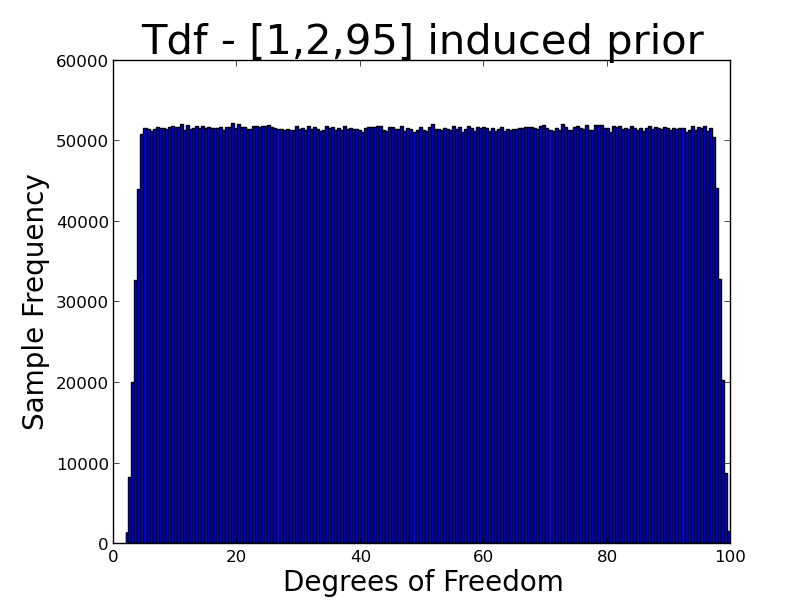
\includegraphics[width=0.8\textwidth]{Tdf1295Prior}
    \caption{Distribution induced by partitioning the prior (uniform-continuous 2 100) into (uniform-continuous 2 95) + (uniform-continuous 0 2) (uniform-continuous 0 1).}
    \label{fig:1295Prior}
\end{figure}

\subsection{Finding a good sum decomposition}
\label{sect:goodSum}
First we look at the expected number of steps needed to reach a neighbourhood of the mode. As explained in Section \ref{section:sampsToMode}, the expected number of steps to $[mode - \epsilon, mode + \epsilon]$ can be analytically computed for the unpartitioned prior (uniform-continuous a b) as $(b-a)/(2\epsilon)$.

For the partitioned priors, we instead perform empirical tests. These tests measure how many samples it takes for different partitions to reach mode neighbourhoods of different sizes. One thousand runs are done for each partition and neighbourhood sizes of of 1, 0.5, 0.2 and 0.02 are considered. The partitions consist of between 2 and 5 values which were drawn with replacement from [0, 0.5, 1, 2, 5, 7, 10, 15, 20, 25, 30, 35, 40, 45].

Table \ref{tab:bestParts} contains the empirical performance for the unpartitioned prior and for the best 2 partitions on each neighbourhood size. We specify partitions in the format (x,y,z) meaning (uniform-continuous 0 x) + (uniform-continuous 0 y) + (uniform-continuous 2 z). All considered partitions respect the constraint $x+y+z = 98$, so that the sum of all the component samples will be in the [2, 100] range specified by the uniform prior of the Tdf model, (uniform-continuous 2 100). 

\begin{table}[h]
  \centering
  \begin{tabular}{lllll}
    \toprule
    \multirow{2}{*}{Partition} & \multicolumn{4}{l}{Target neighbourhood size} \\
    \cmidrule(r){2-5} 
    & 1 & 0.5 & 0.2 & 0.02 \\
    \midrule
    Unpartitioned & 98.38 & 199.29 & 494.87 & 4919.75 \\
    (5, 93) & 89.03 & 122.87 & 172.9  & 670.14 \\
    (20, 78)& 92.55 & 142.6  & 259.21 & 1834.18 \\
    (2, 96) & 92.56 & 117.35 & 157.83 & 371.9 \\
    (1, 45, 52) & 123.97 & 146 & 172.78 & 400.01 \\
    (0.5, 2, 95.5) & 134.24 & 162.03 & 201.57 & 297.79 \\
    (1, 2, 95) & 130.06 & 155.48  & 186.83 & 317.31 \\
    \bottomrule
  \end{tabular}
  \caption{Expected number of steps to mode neighbourhoods on the Tdf continuous model for an unpartitioned prior and some of the best sum decomposition priors.}
  \label{tab:bestParts}
\end{table}

The best partition depends on the size of the neighbourhood, but we can observe partitions that consistently and significantly outperform the unpartitioned prior on all the neighbourhood sizes looked at above. In fact, for epsilon values of 0.1 and 0.01 the unpartitioned prior performs worse than any of the partitioned variants. Additionally, as epsilon gets smaller, it becomes useful to have smaller partition components. This leads to the 0.5 partition appearing in the best solution for a mode neighbourhood of size 0.02, but not in any of the top solutions for larger neighbourhoods.

The second aspect of convergence that a partition might help with is the mixing rate around the mode. In order to test the priors' mixing properties we need to consider what happens after the markov chain reaches the mode. We do this by setting the initial sample to the mode of the true posterior distribution and checking how much the chain moves over the next 1000 samples. Repeating this test 100 times and averaging the sum of absolute jump distances gives us the results in Table \ref{tab:partMix}.

\begin{table}[h]
  \centering
  \begin{tabular}{lll}
    \toprule
    Partition & Mean distance travelled & Variance in distance travelled \\
    \midrule
    Unpartitioned & 7.75 & 13.43 \\
    (1, 1, 1, 95) & 137.55 & 393.96 \\
    (1, 1, 1, 1, 94) & 135.08 & 616.41 \\
    (1, 1, 2, 94) & 131.19 & 539.03 \\
    (1, 1, 1, 2, 93) & 129.91 & 583.16 \\
    (0.5, 1, 1, 1, 94.5) & 126.76 & 382.09 \\
    (1, 2, 95) & 125.67 & 408.16 \\
    (1, 1, 96) & 125.44 & 311.76 \\
    (0.5, 1, 2, 94.5) & 123.38 & 487.26 \\
    (1, 1, 2, 2, 92) & 122.9 & 615.54 \\
    (2, 2, 94) & 121.25 & 844 \\
    \bottomrule
  \end{tabular}
  \caption{Average distance travelled around the mode on the Tdf continuous model for an unpartitioned prior and some of the best sum decomposition priors.}
  \label{tab:partMix}
\end{table}

This test only measures the average distance travelled (i.e. sum of absolute differences between consecutive samples), which could be a misleading measure of mixing. However, the large difference between the unpartitioned and the partitioned variants do suggest that there is some improvement here. We perform further tests on the mixing rate in Section \ref{sect:1295Eval}.

Based on the above results, we decide to further investigate the performance of the (1, 2, 95) partitioned prior, since this decomposition performs well both in reaching the mode and in mixing around it.

\subsection{Evaluating the (1,2,95) sum decomposition}
\label{sect:1295Eval}

Table \ref{tab:bestParts} makes clear the increased speed in reaching a neighbourhood of the mode offered by the decompositions. The potential benefit conferred in mixing rate is less clear however. To test this we look at the sample evolution (Figure \ref{fig:tdfPSampEvol}) and autocorrelation plots (Figure \ref{fig:tdfPAutoCorr}) for two runs obtained with an unpartitioned and a (1,2,95) partitioned prior. These experiments confirm our preliminary results from Section \ref{sect:goodSum}, and show that the partitioned prior does help with mixing around the mode and with eliminating large correlations between consecutive samples. 

\begin{figure}[h]
    \centering
    \begin{subfigure}[t]{0.48\textwidth}
      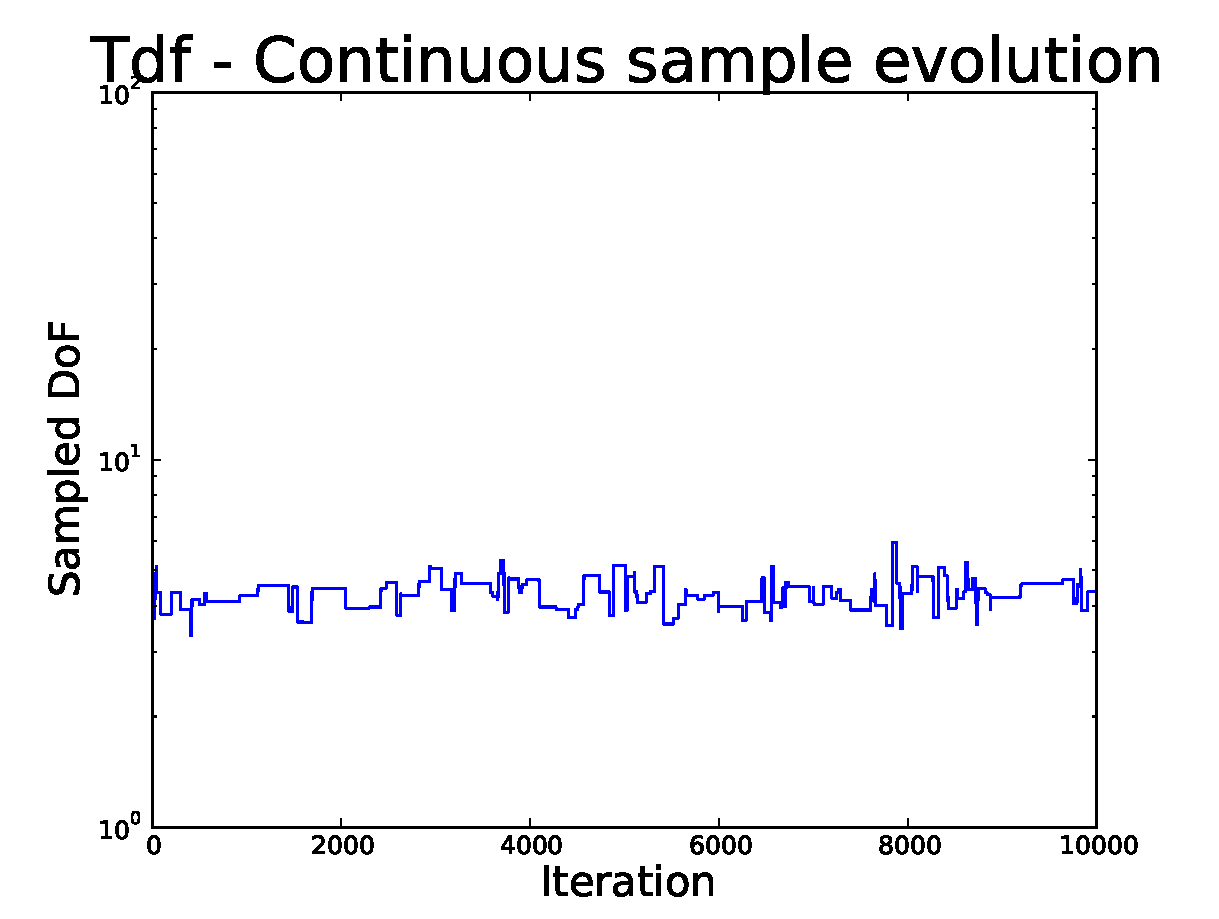
\includegraphics[width=\textwidth]{TdfSampEvol}
    \end{subfigure}
    ~
    \begin{subfigure}[t]{0.48\textwidth}
      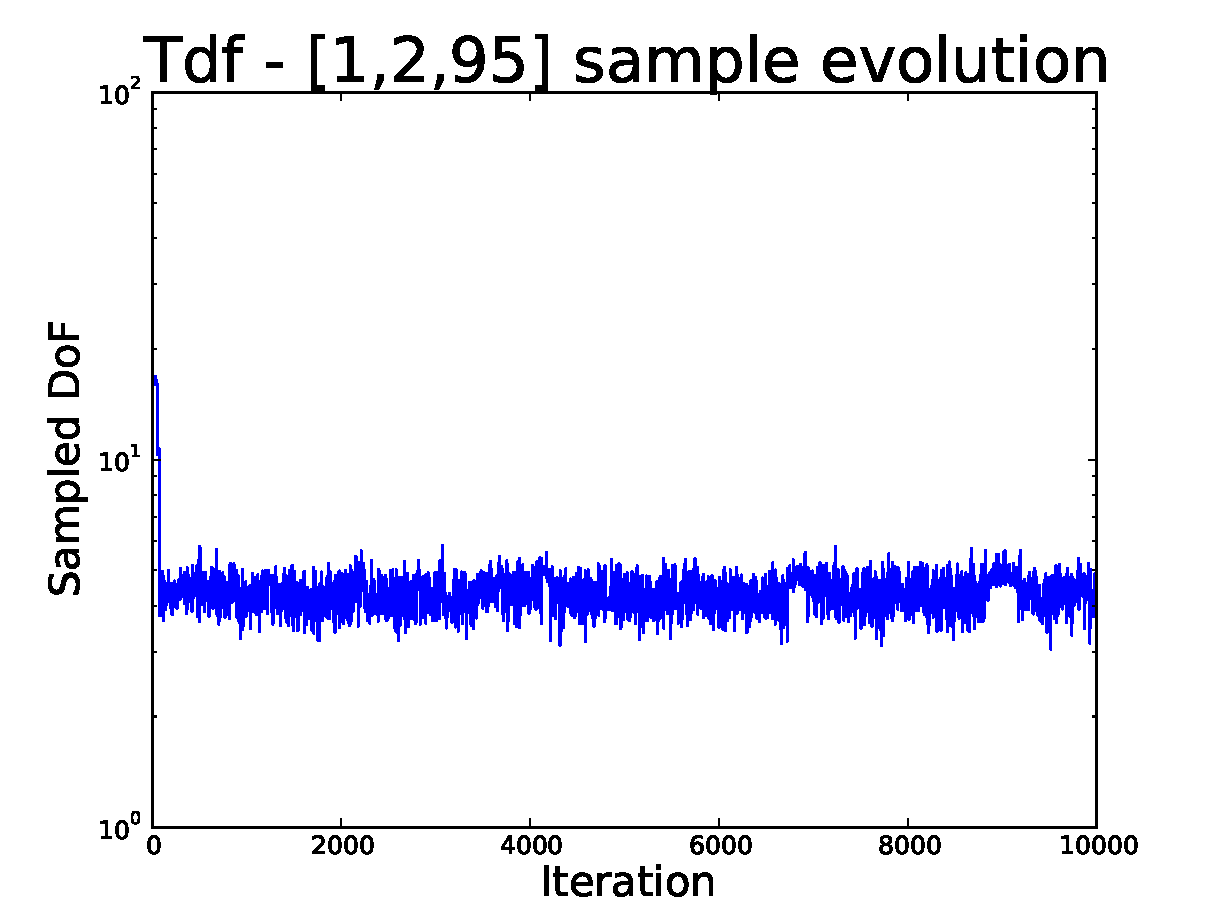
\includegraphics[width=\textwidth]{Tdf1295SampEvol}
    \end{subfigure}
    \caption{Sample evolutions for the unpartitioned and the (1, 2, 95) partitioned priors, over 10,000 samples on the Tdf continuous model.}
    \label{fig:tdfPSampEvol}
\end{figure}

\begin{figure}[h]
    \centering
    \begin{subfigure}[t]{0.48\textwidth}
      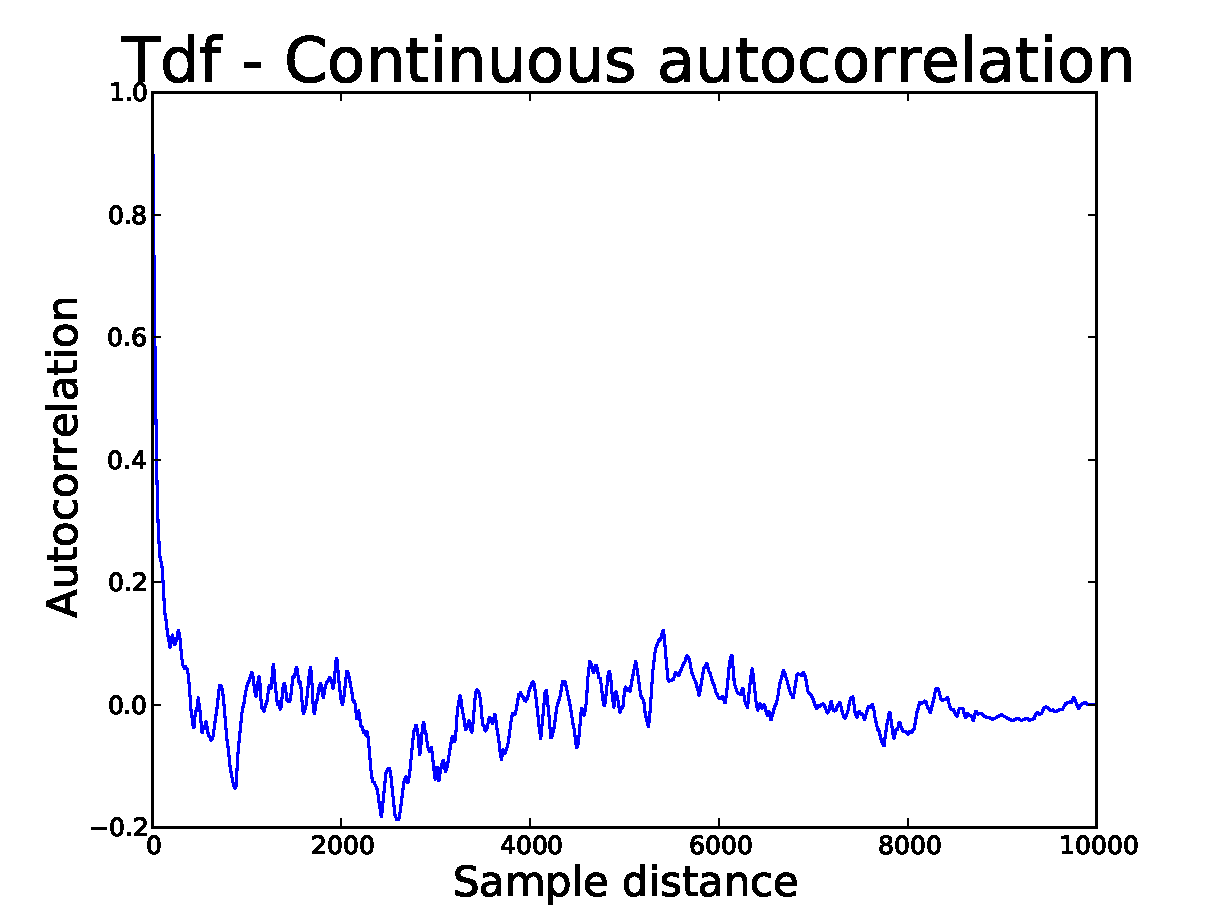
\includegraphics[width=\textwidth]{TdfAutoCorr}
    \end{subfigure}
    ~
    \begin{subfigure}[t]{0.48\textwidth}
      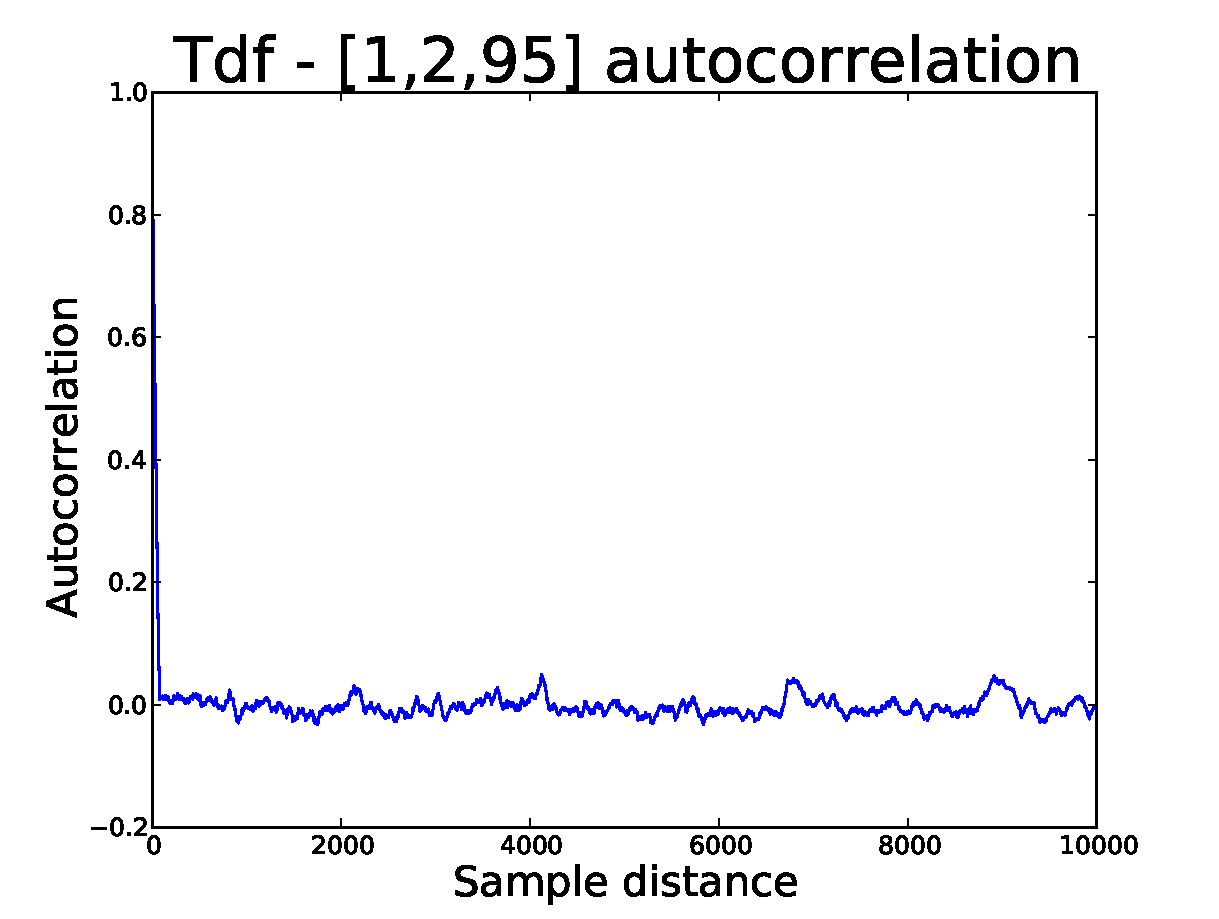
\includegraphics[width=\textwidth]{Tdf1295AutoCorr}
    \end{subfigure}
    \caption{Sample autocorrelations for the unpartitioned and the (1, 2, 95) partitioned priors, over 10,000 samples on the Tdf continuous model.}
    \label{fig:tdfPAutoCorr}
\end{figure}

The final test in determining the quality of the decomposition is to look at the actual sample distributions obtained under the two different prior formulations . For convenience, the true posterior for the Tdf continuous model is shown again in Figure \ref{fig:tdfPLL}. Looking at the sample distributions in Figure \ref{fig:tdfPDist} it is quite clear the partitioned prior outperforms the original, unpartitioned, variant. However, this result may be misleading since we are evaluating it on the same distribution which we used to choose the form of the partition. To test the robustness of our partition we repeat the above tests on a new model.

\begin{figure}[h]
    \centering
    \begin{subfigure}[t]{0.48\textwidth}
      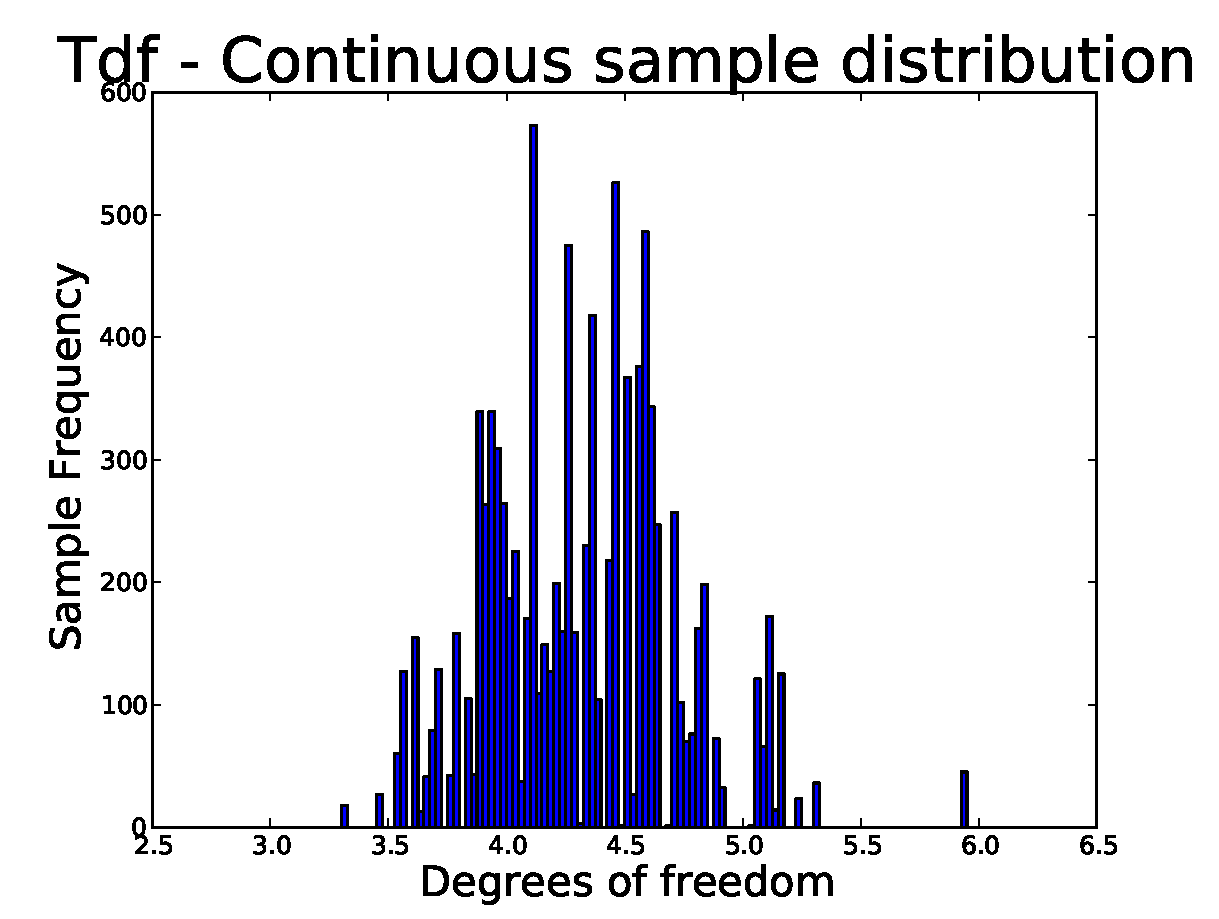
\includegraphics[width=\textwidth]{TdfSampDist}
    \end{subfigure}
    ~
    \begin{subfigure}[t]{0.48\textwidth}
      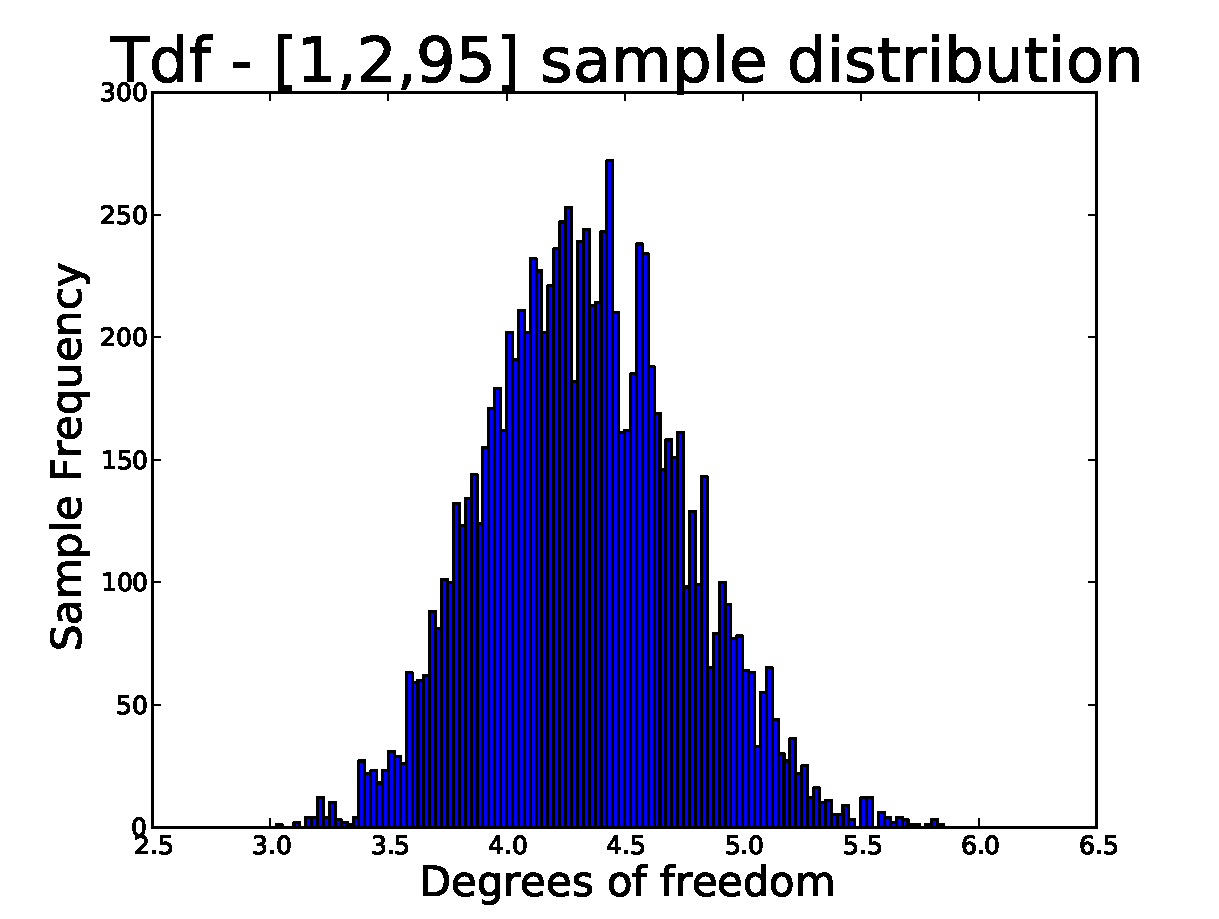
\includegraphics[width=\textwidth]{Tdf1295SampDist}
    \end{subfigure}
    \caption{Sample distributions for the unpartitioned and the (1, 2, 95) partitioned priors, over 10,000 samples on the Tdf continuous model.}
    \label{fig:tdfPDist}
\end{figure}

\subsubsection{The Tdf21 model}
In order to test our decomposition on a different posterior distribution, we generate 1,000 datapoints from a Student t distribution with 21 degrees of freedom and condition the Tdf Continuous model on this new dataset. The resulting posterior is shown in Figure \ref{fig:tdfPPost}. The mode here is actually 11.5. This is probably due to the fact that 1000 datapoints are not enough to accurately pinpoint a student-t with so many degrees of freedom (21) since, as the number of degrees of freedom increases, the differences between corresponding student-t distributions shrinks. The posterior distribution is however significantly different from the one for the previous dataset, which should be sufficient for testing the properties of the priors.

\begin{figure}[h]
    \centering
    \begin{subfigure}[t]{0.48\textwidth}
      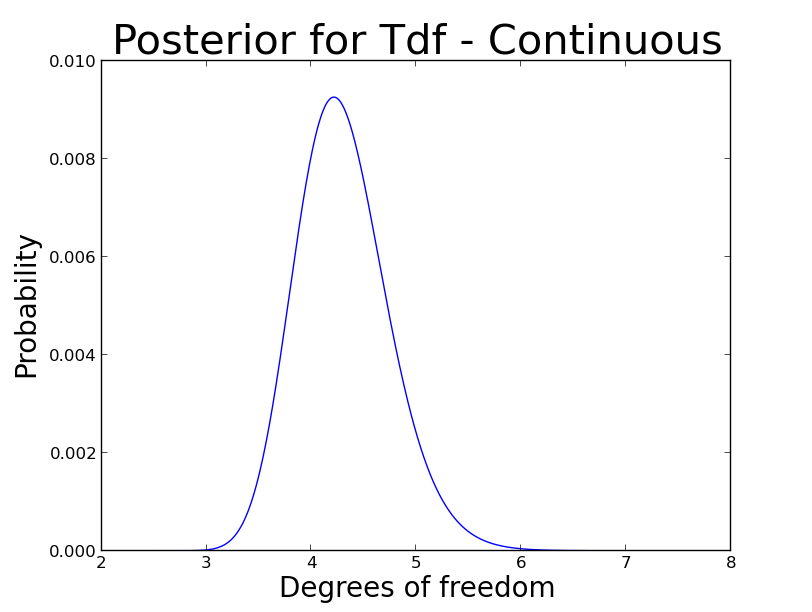
\includegraphics[width=\textwidth]{TdfContPost}
    \end{subfigure}
    ~
    \begin{subfigure}[t]{0.48\textwidth}
      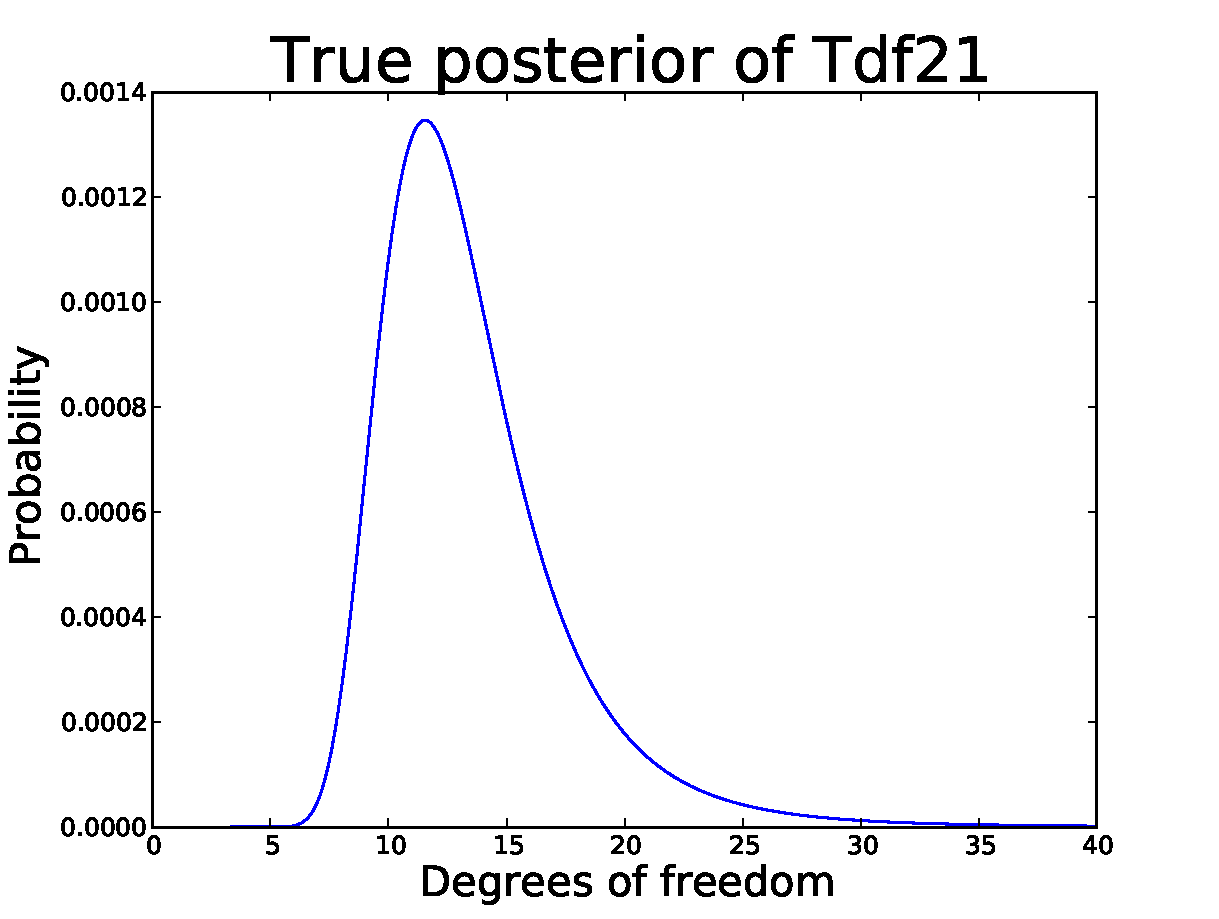
\includegraphics[width=\textwidth]{Tdf21Post}
    \end{subfigure}
    \caption{The true posteriors of the Tdf continuous and the Tdf21 continuous models.}
    \label{fig:tdfPPost}
\end{figure}

In order to better understand how the Metropolis-Hastings algorithm will be affected by this change, Figure \ref{fig:tdfPLL} also shows the log-likelihoods induced by the original Tdf Continuous model and by the Tdf21 continuous model. We can see that the Tdf21 log-likelihood is much flatter than the one for the original model. By repeating the mixing tests performed above we can test the effect of this difference.

\begin{figure}[h]
    \centering
    \begin{subfigure}[t]{0.48\textwidth}
      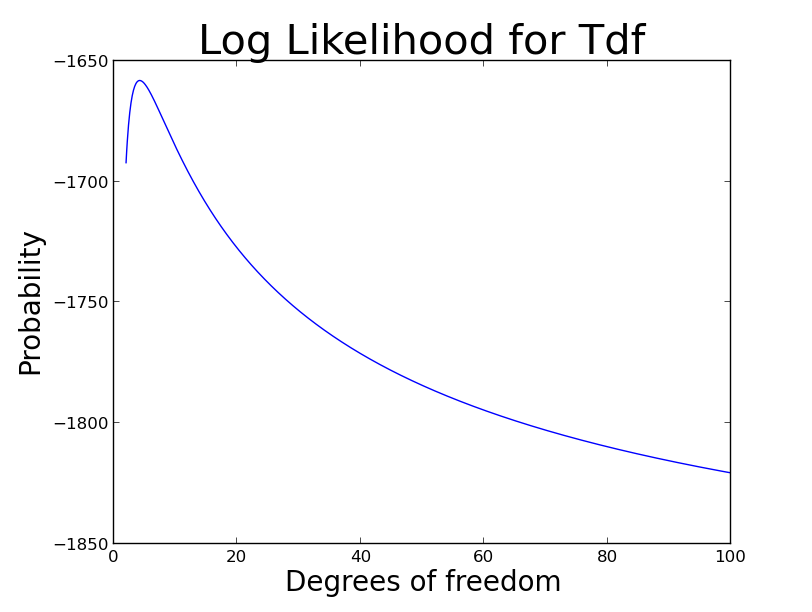
\includegraphics[width=\textwidth]{TdfContLL}
    \end{subfigure}
    ~
    \begin{subfigure}[t]{0.48\textwidth}
      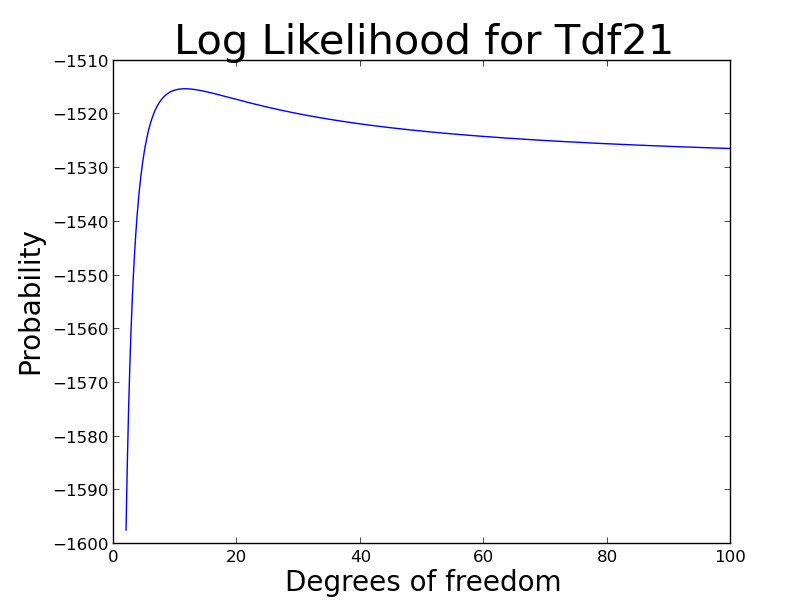
\includegraphics[width=\textwidth]{Tdf21LL}
    \end{subfigure}
    \caption{The true log-likelihoods of the Tdf continuous and the Tdf21 continuous models.}
    \label{fig:tdfPLL}
\end{figure}

\subsubsection{Evaluating the decomposition on the Tdf21 model}
We now test the convergence of the priors on the Tdf21 model by plotting the sample evolution, the sample autocorrelation and the sample distributions. The partitioned prior is the same one we used on the previous datapoints, namely (1,2,95). From the sample evolutions (Figure \ref{fig:tdf21PSampEvol}) we can see that the partitioned samples tend to clump a little more since bigger changes in the samples only occur when the 95 component changes. Both versions seem to mix well though.


\begin{figure}[h]
    \centering
    \begin{subfigure}[t]{0.48\textwidth}
      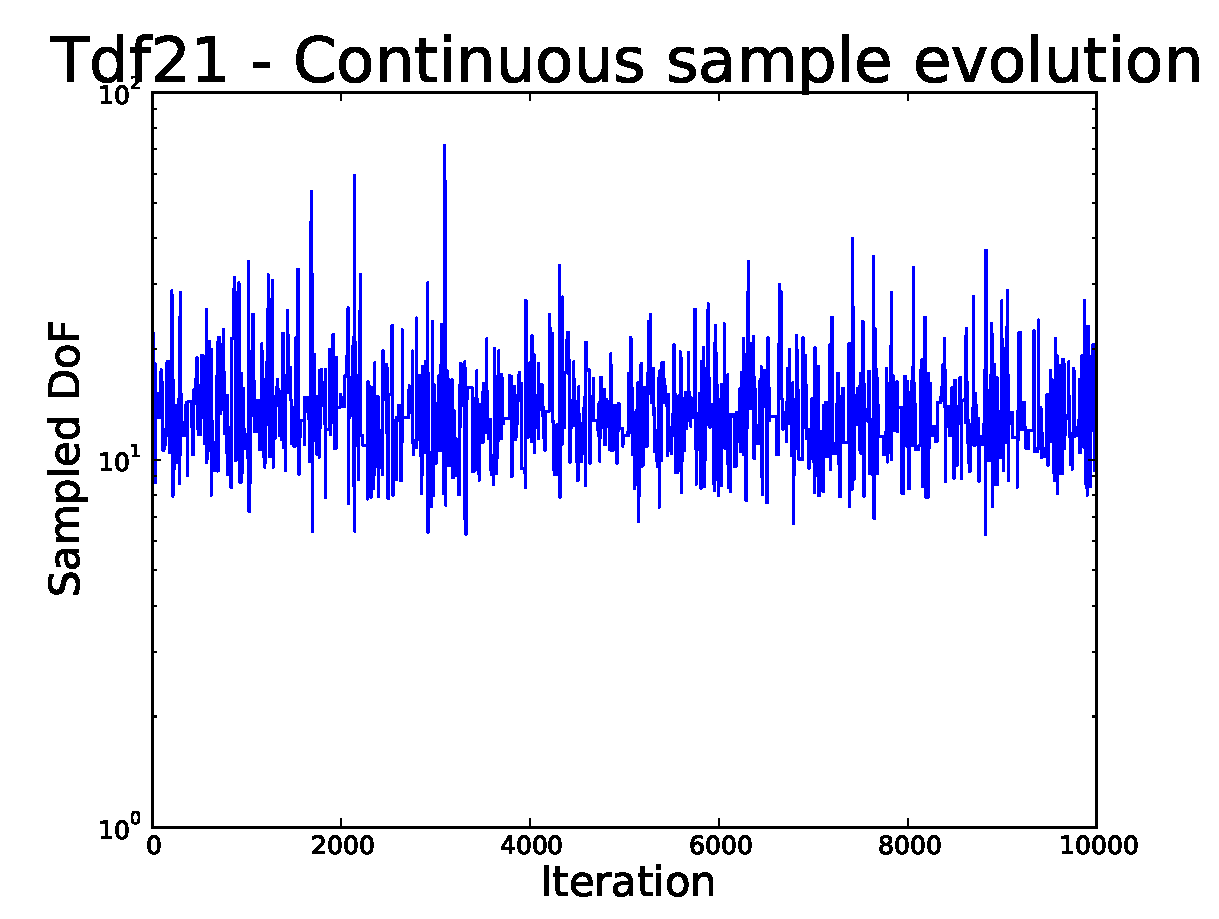
\includegraphics[width=\textwidth]{Tdf21SampEvol}
    \end{subfigure}
    ~
    \begin{subfigure}[t]{0.48\textwidth}
      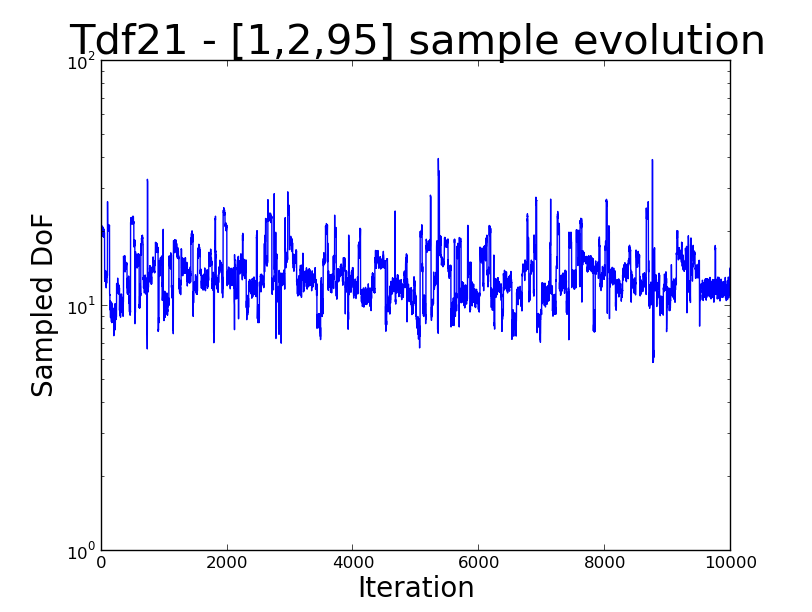
\includegraphics[width=\textwidth]{Tdf211295SampEvol}
    \end{subfigure}
    \caption{Sample evolutions for the unpartitioned and the (1, 2, 95) partitioned priors, over 10,000 samples on the Tdf21 model.}
    \label{fig:tdf21PSampEvol}
\end{figure}

The autocorrelation plots shown in Figure \ref{fig:tdf21PAutoCorr} are also more similar than in the case of the original Tdf model. The unpartitioned prior does quite well here since the flat shape of the log-likelihood means there is a higher chance that a proposition drawn from the prior will be accepted by the Metropolis-Hastings algorithm.

\begin{figure}[h]
    \centering
    \begin{subfigure}[t]{0.48\textwidth}
      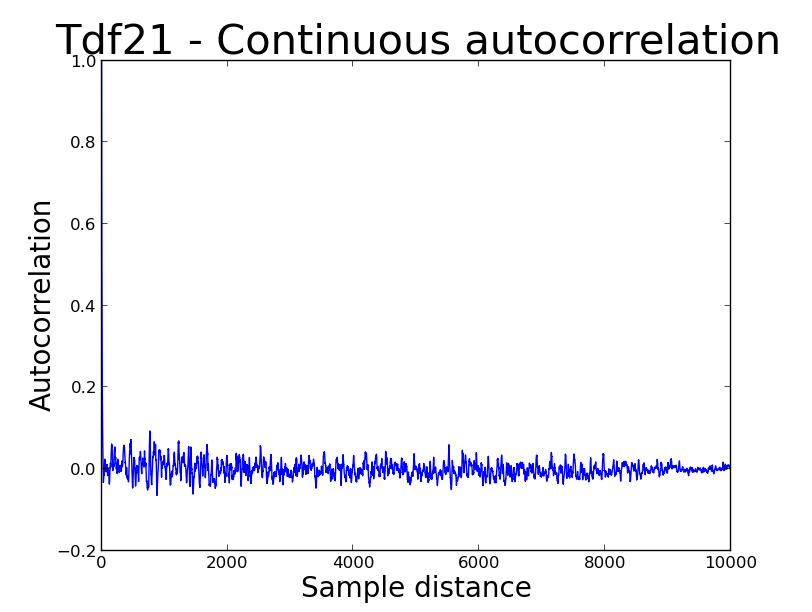
\includegraphics[width=\textwidth]{Tdf21AutoCorr}
    \end{subfigure}
    ~
    \begin{subfigure}[t]{0.48\textwidth}
      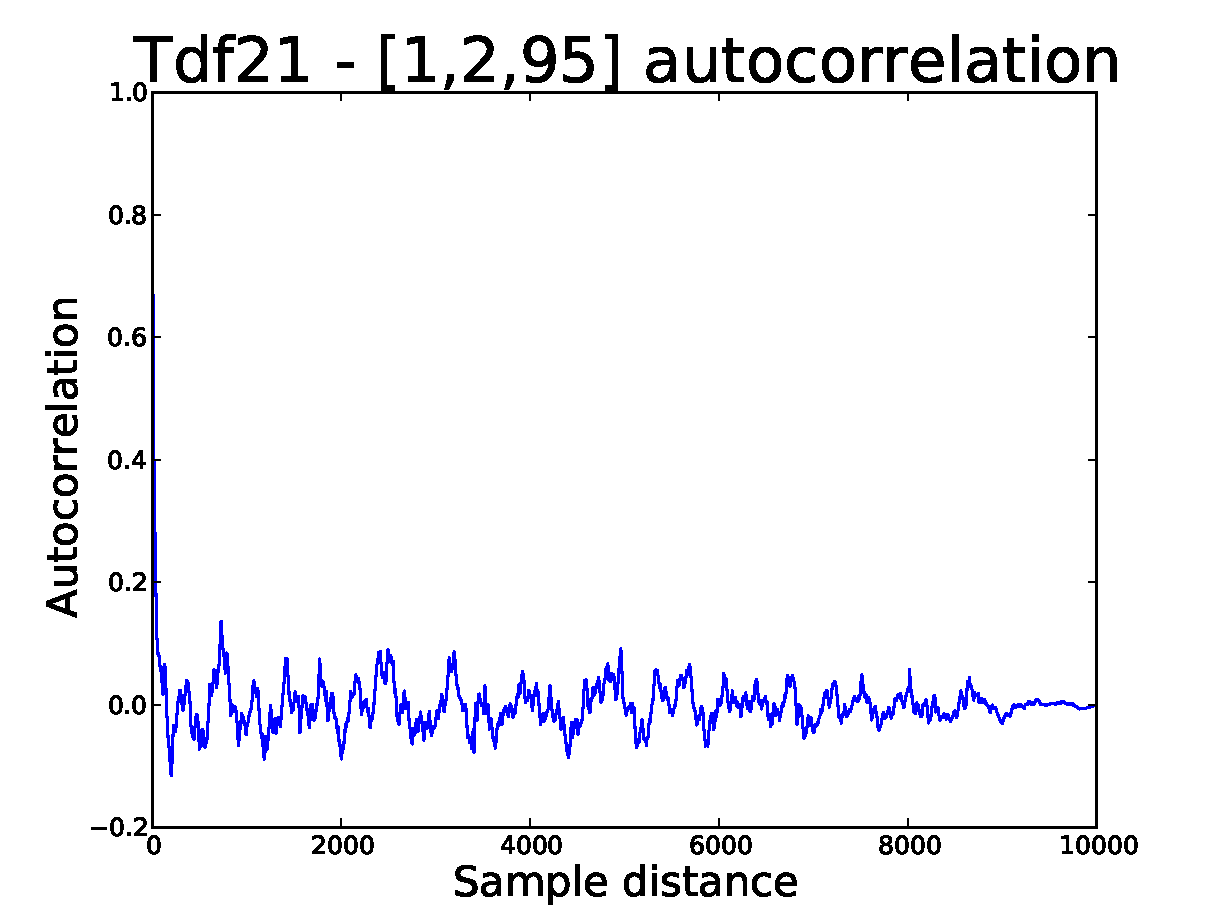
\includegraphics[width=\textwidth]{Tdf211295AutoCorr}
    \end{subfigure}
    \caption{Sample autocorrelations for the unpartitioned and the (1, 2, 95) partitioned priors, over 10,000 samples on the Tdf21 model.}
    \label{fig:tdf21PAutoCorr}
\end{figure}

Finally, Figure \ref{fig:tdf21PSampDist} shows the sample distributions. Here we can see that, despite the similar performance of the two priors on the mixing tests, the partitioned prior still results in a significantly smoother distribution.

\begin{figure}[h]
    \centering
    \begin{subfigure}[t]{0.48\textwidth}
      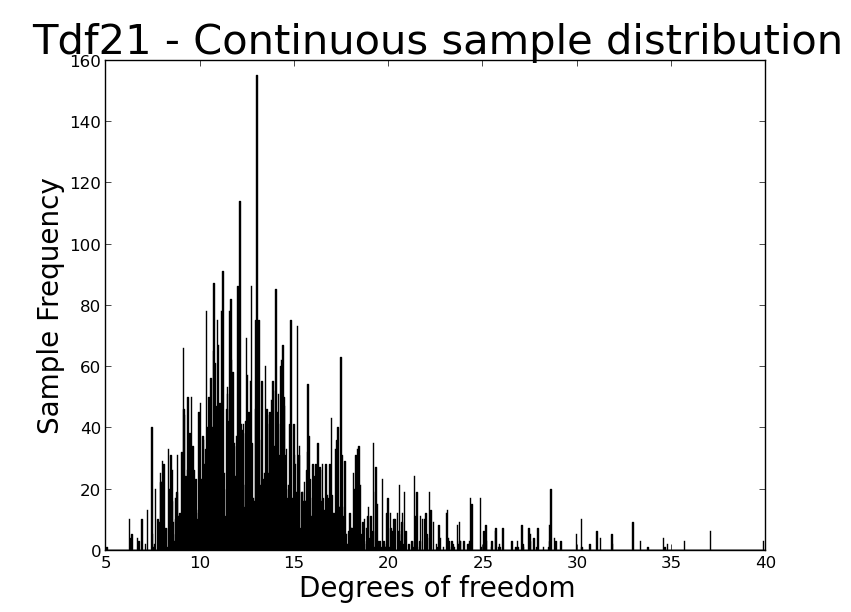
\includegraphics[width=\textwidth]{Tdf21SampDist}
    \end{subfigure}
    ~
    \begin{subfigure}[t]{0.48\textwidth}
      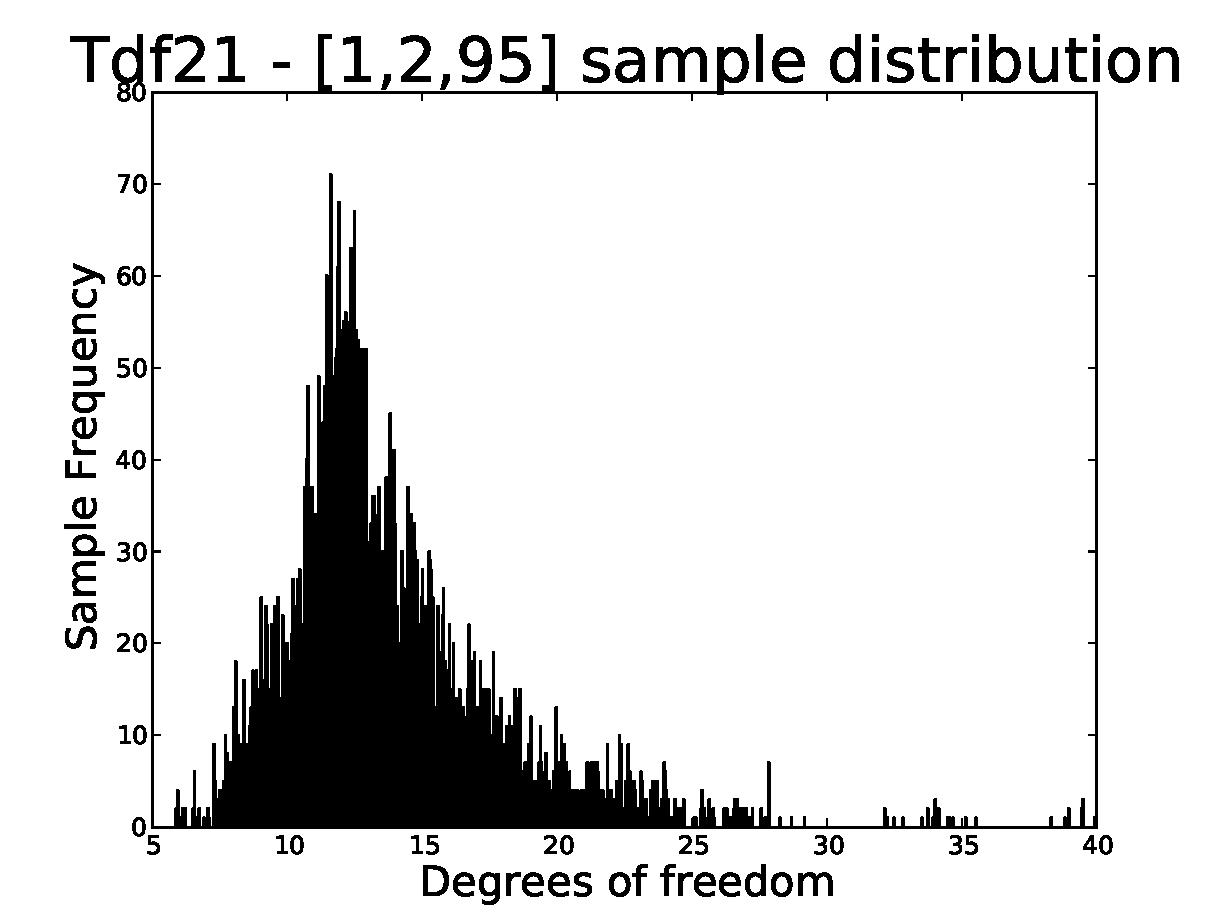
\includegraphics[width=\textwidth]{Tdf211295SampDist}
    \end{subfigure}
    \caption{Sample distributions for the unpartitioned and the (1, 2, 95) partitioned priors, over 10,000 samples on the Tdf21 model.}
    \label{fig:tdf21PSampDist}
\end{figure}

\section{Bit decomposition}
\label{sect:bitDecomp}
As mentioned in Section \ref{sect:sumUnif}, one problem with the sum of uniforms decomposition is that it alters the shape of a uniform prior. We would like to come up with decompositions that leave uniform priors invariant and that could therefore be applied indescriminately to re-write probabilistic programs containing such distributions. A family of invariant partitions of an uniform prior can be constructed by thinking in terms of the bit representation of the uniform samples. In order to be able to represent any real number, we can consider a bit representation of the number up to a certain prevision and then add a single uniform-continuous value to the bit's value. 

\subsection{Definition}
In order to partition any uniform interval (uniform-continuous a b) it is sufficient to be able to partition the interval (uniform-continuous 0 1). Once this is accomplished, the target interval can be obtained through the transformation: (uniform-continuous a b) = a + (b-a) * (uniform-continuous 0 1).

In order to partition the interval (uniform-continuous 0 1) we first pick a bit depth, k, such that $ k \in \{ 0, 1, \ldots \infty \} $ We then define (uniform-continuous 0 1) $= flip*2^{-1} + flip*2^{-2} \ldots + flip*2^{-k} +$ (uniform-continuous 0 $2^{-k}$), where flip is a function which flips a coin and returns 0 or 1 with probability 1/2 each.

\subsection{Evaluation on Tdf and Tdf21}

To get an idea of the properties of bit decomposition we perform empirical evaluations on the Tdf and Tdf21 continuous models. Looking at the sample distributions in Figures \ref{fig:tdfPSampDist} and \ref{fig:tdf21PSampDist} we can see that a 3rd degree bit decomposition obtains similar performance to an unpartitioned prior. Intuitively this is because we are still subjecting proposals to the Metropolis-Hastings acceptance ratio, so if our program decides to flip one of the leading bits the proposal will be rejected, leading to bad mixing. As the depth of the bit decomposition increases, however, the probability that one of the leading bits is picked diminishes and therefore we will expect the mixing rate to improve. \todo{Should be possible to give some more formal results here.} We, however, restrict ourselves to a 3rd degree decomposition here since a higher degree variant would exhibit the problem ``stuck samples'', which is discussed in Section \ref{sect:stuckSamples}.

\begin{figure}[h]
    \centering
    \begin{subfigure}[t]{0.48\textwidth}
      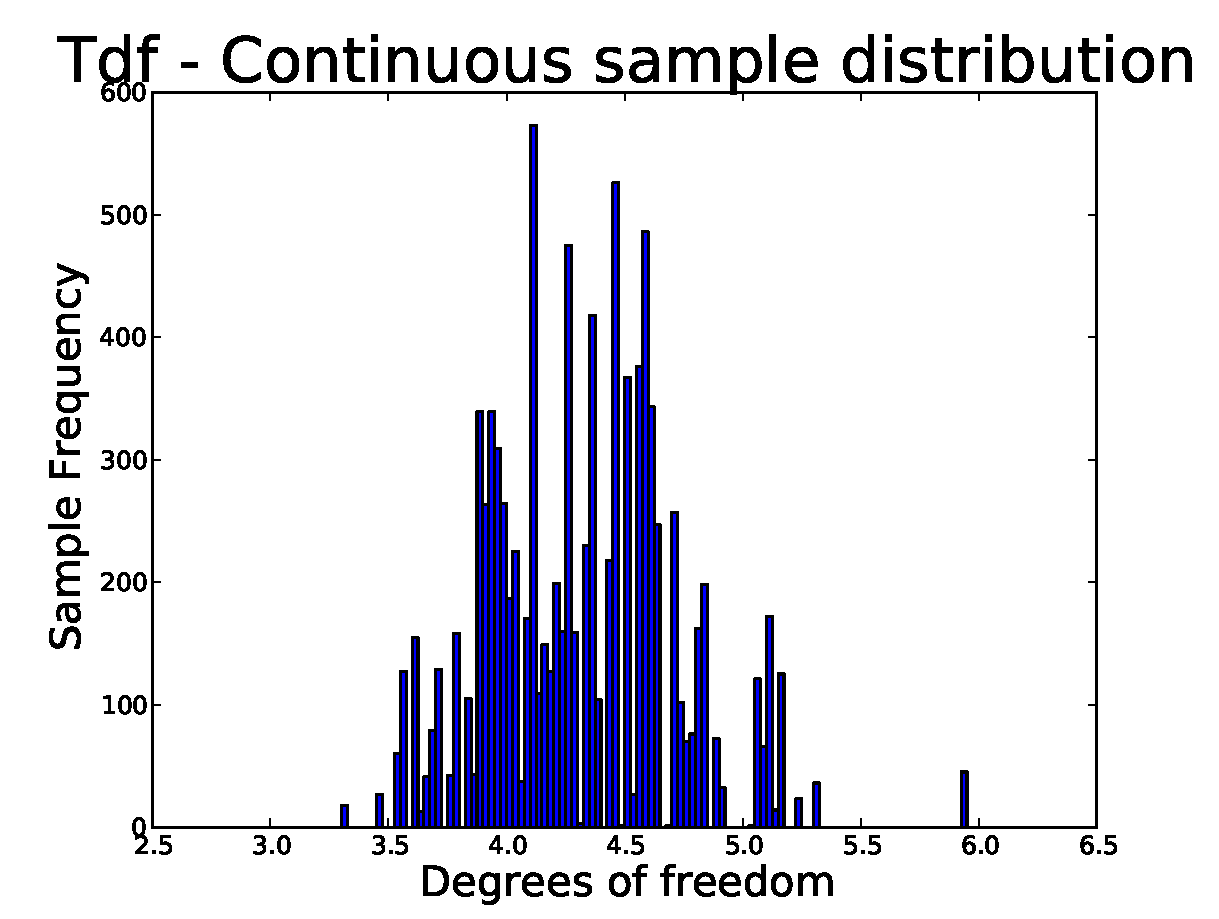
\includegraphics[width=\textwidth]{TdfSampDist}
    \end{subfigure}
    ~
    \begin{subfigure}[t]{0.48\textwidth}
      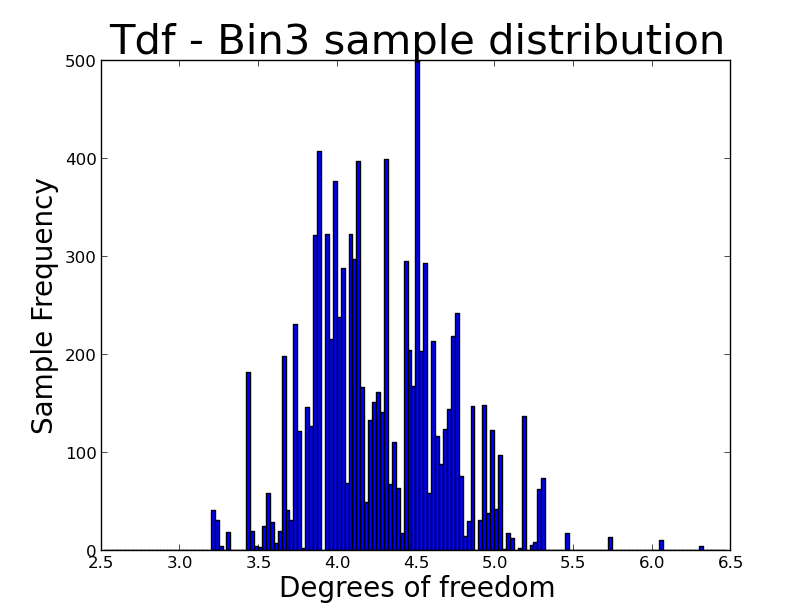
\includegraphics[width=\textwidth]{TdfBin3SampDist}
    \end{subfigure}
    \caption{Sample distributions for an unpartitioned and a 3 bit decomposition prior, over 10,000 samples on the Tdf continuous model.}
    \label{fig:tdfPSampDist}
\end{figure}

\begin{figure}[h]
    \centering
    \begin{subfigure}[t]{0.48\textwidth}
      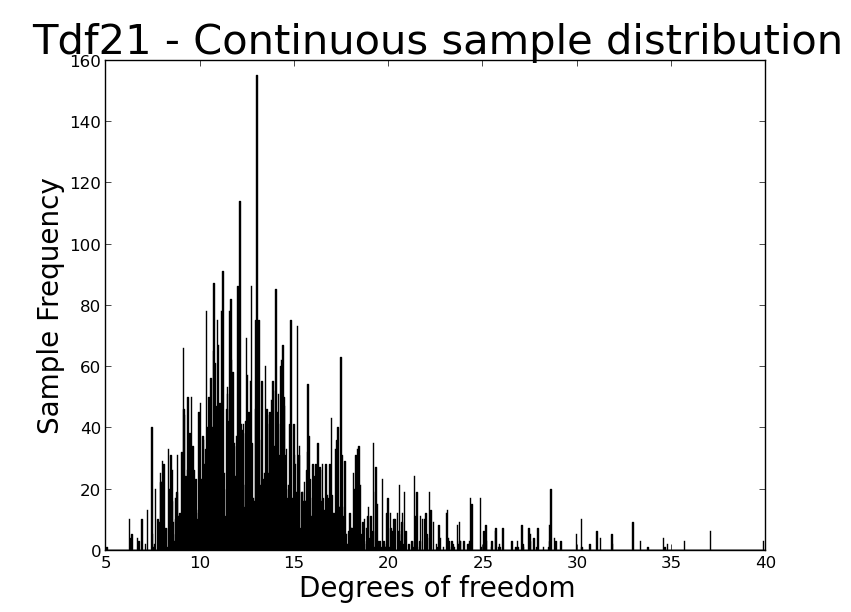
\includegraphics[width=\textwidth]{Tdf21SampDist}
    \end{subfigure}
    ~
    \begin{subfigure}[t]{0.48\textwidth}
      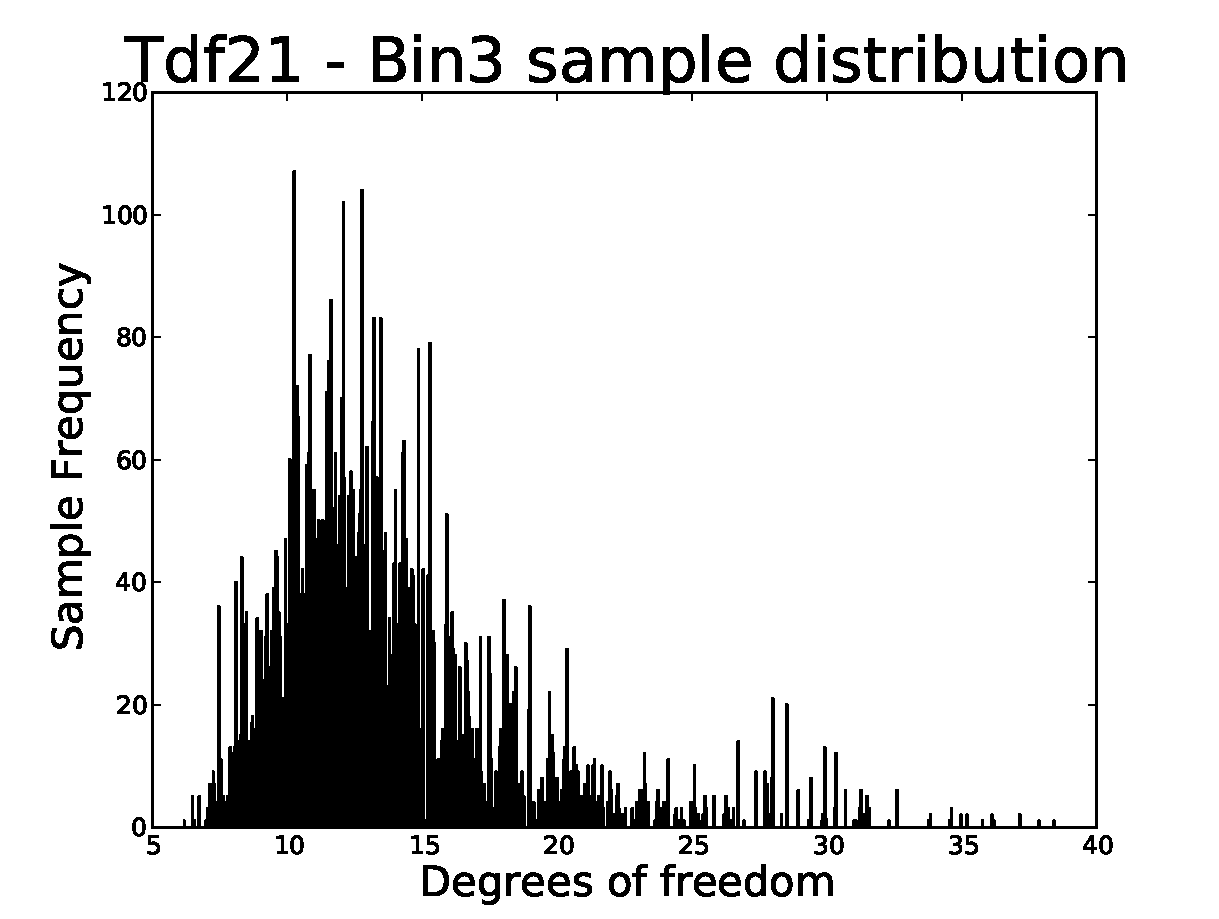
\includegraphics[width=\textwidth]{Tdf21Bin3SampDist}
    \end{subfigure}
    \caption{Sample distributions for an unpartitioned and a 3 bit decomposition prios, over 10,000 samples on the Tdf21 model.}
    \label{fig:tdf21PSampDist}
\end{figure}

The expected time to reach a mode neighbourhood is analyzed in Table \ref{tab:bestParts}. Here we can see that the 3rd degree binomial provides a significant improvement over the unpartitioned prior, though not as significant as the sum of uniforms does. \todo{talk about how binomials of different depth perform here}. On the depth 7 bit decomposition, we see good results on the small neighbourhoods but erratic ones on the larger neighbourhoods. The reason is again the fact that bit decompositions can result in ``stuck samples'', which are discussed in Section \ref{sect:stuckSamples}.

\begin{table}[H]
  \centering
  \begin{tabular}{llllll}
    \toprule
    \multirow{2}{*}{Model} & \multirow{2}{*}{Partition} & \multicolumn{4}{l}{Target neighbourhood size} \\
    \cmidrule(r){3-6} 
    & & 1 & 0.5 & 0.2 & 0.02 \\
    \midrule
    Both & Unpartitioned & 98 & 196 & 490 & 4900 \\
    \midrule
    \multirow{3}{*}{Tdf Continuous} & (1, 2, 95) & 130.06 & 155.48  & 186.83 & 317.31 \\
    & Bit 3 & 52 & 95.3  & 272.6 & 2232.4 \\
    & Bit 7 & 1080.78 & 866.64 & 776.26 & 1433.37 \\
    \midrule
    \multirow{3}{*}{Tdf21 Continuous} & (1, 2, 95) & 93.5 & 128.8  & 173.9 & 714.98 \\
    & Bit 3 & 117.52 & 170.65  & 401.5 & 2969.9 \\
    & Bit 7 & 161.86 & 177.22 & 284.99 & 1739.84 \\
    \bottomrule
  \end{tabular}
  \caption{Expected number of steps to neighbourhoods of the mode on the Tdf and Tdf21 continuous models for an unpartitioned prior, the (1,2,95) sum decomposition and 2 bit decompositions.}
  \label{tab:bestParts}
\end{table}

\subsection{Getting stuck on a bad sample}
\label{sect:stuckSamples}
A problem with the bit decomposition is that it is possible to construct scenarios in which a sample will get stuck and be arbitrarily unlikely to reach a particular neighbourhood of the mode. One simple such scenario can be constructed by assuming a guiding posterior log-likelihood that is convex, symmetric around the mode and steep enough that the probability of a sample moving significantly further away from the mode is negligible.

The simplest example of getting stuck can be observed by considering the bit decomposition of depth 1: (uniform-continuous 0 1) = $flip*2^{-1} +$ (uniform-continuous 0 $2^{-1}$). In this case, if the the mode is in the interval $[0.5 + \epsilon , 0.75]$, and $[mode - \epsilon, mode + \epsilon]$ is the mode neighbourhood we want to reach, then it is possible for the prior to get stuck outside of our target neighbourhood.
 
A concrete example would be:
\begin{flalign*}
  &\text{(uniform-continuous 0 1)} = flip*2^{-1} + \text{(uniform-continuous 0 }2^{-1})& \\
  &\quad\quad\quad\quad mode \sim 0.6 &\\
  &\quad\quad\quad\quad \epsilon \sim 0.05 &\\
  &\quad\quad\quad\quad flip \sim 0 &\\
  &\quad\quad\quad\quad \text{(uniform-continuous 0 }2^{-1}) \sim 0.4 &
\end{flalign*}

In this case, setting flip to $1$ would be very likely rejected since jumping from $0.4$ to $0.4 + 0.5 = 0.9$ takes us much further away from the mode at $0.6$ then we currently are. Further the uniform is likely to only accept resampled values in the $(0.4, 0.5)$ interval, which won't change the above situation. In order for us to get unstuck we would need either a very unlikely bit flip to be accepted or the uniform to accept a very unlikely resample close to 0, which could then be followed by a bit flip. Assuming we can make the log-likelihood arbitrarily steep around the mode, then we can expect to be stuck in this local optimum for an arbitrarily long number of samples.

Some possible solutions to avoid getting stuck would be:
\begin{itemize}

\item
Having the option of changing multiple bits at a time (eg: sample a variable to determine how many bits to change). This would ensure there are no hard local maximas. However, situations would still arise where a large number of bits would need to be concurrently changed to specific values in order for a sample to be accepted, which means we might still be stuck in a certain position for a long time untill just the right combination of bits is picked. \todo{is a more thorough analysis feasible here?}

\item
Using multiple shifted variants of the prior, where shifting by $shift$ means mapping sample $x$ to $(x + shift)\%1$). It can be shown that a single shift is enough to avoid getting stuck. However the effect on performance of adding shifts is complex, since performing a shift in an unstuck position can lead to us moving further away from the mode. More analysis of the effect of shifts is presented in \ref{sect:shifts}.

\item
Using multiple variants of the prior with different bit depths. If a sample is stuck on bit b, then moving it into a prior with depth < b will unstick it. However, this will result in the bits with the highest values being resampled more often, since they will be present in the most priors, which will have a negative effect on the mixing benefits offered by the decomposition. \todo{add more analysis on this}

\end{itemize}

One idea that is tempting but incorrect is to determine, with some likelihood, when a certain markov chain has become stuck based on its sample history. This would allow us to explicitly correct for the chain getting stuck. We could toss a coin to decide if we think we're currently stuck and if we decided we were not stucj we could sample normally. If we did think we were stuck, we could determine in which bits we might be stuck and pick one of these. We could then determine the interval in which the mode should be if we were indeed stuck on the bit we picked and sample uniformly from that interval.

This approach is atractive because, for the kth bit $flip*2^{-k}$, the target interval we would determine the mode to be in would be of size $2^{-k-1}$. However, the problem with this idea is that it isn't just picking proposals from a static prior or proposal kernel, but the proposal pattern is actually influenced by the shape of the log likelihood. \todo{explain why this is wrong}

\subsection{Mixtures of shifted bit decompositions}
\label{sect:shifts}
In this section we explore two variants of the mixture of shifted bits. First we look at what is necessary simply to ensure that we'll never get stuck. Second we look at what is needed to be able to move from any stuck position to a neighbourhood of the mode in one jump. This second variant ends up providing better performance.

\subsubsection{Avoiding getting stuck}
\label{sect:stuckMath}
\todo{not sure if this section is clear enough. add diagrams?}

It turns out that a mixture of 2 bit decompositions, one of which is a shifted variant of the other, is sufficient to ensure that it is impossible to get stuck. However it seems we need to use a mixture of K priors in order to ensure that the binomial of depth K can move from any stuck position to the mode in one step. 

To better understand how these shifts work, we consider the formulation:
\begin{flalign*}
  &total = flip1*0.5 + flip2*0.25 + \text{(uniform-continuous 0 0.25)}& \\
  &\hspace{3em} flip1 \sim 0& \\
  &\hspace{3em} flip2 \sim 1& \\
  &\hspace{3em} \text{(uniform-continuous 0 0.25)} \sim \epsilon& \\
  &=> total = 0.25 + \epsilon \tag{$\epsilon$ is an arbitrarily small positive number}&
\end{flalign*}

Here we are stuck since, in order to reach the mode, we need to switch the $flip2$ bit to 0, but this flip will be rejected as it would mean moving significantly further away from the mode than we currently are. We want to determine what size of a shift needs to exist in order for us to be able to become unstuck. 

For any shift $s$ we choose, the shifted prior will be:
\[ shiftTotal = (s + total) \% 1 = (s + 0.25 + \epsilon) \% 1 \] 
And flipping the second bit ($flip2$) to 0 would result in a proposal:
\[proposal = s + \epsilon\]

We can now show that, if a shift is too small, then the proposal will be rejected. Specifically:
\begin{flalign*}
&\text{If } & \\
&\hspace{3em}mode = 0.25 - \epsilon &\\
&\hspace{3em} s < 0.125 - 2*\epsilon &\\
&\text{Then } & \\
&\hspace{3em} |shiftTotal - mode| = |s + 0.25 + \epsilon - 0.25 + \epsilon| = s + 2*\epsilon < 0.125 &\\
&\hspace{3em} |proposal - mode| = | s + \epsilon - 0.25 + \epsilon | = 0.25 - s + 2*\epsilon > 0.125 &\\
&=> distance(proposal, mode) > distance(shiftTotal, mode) \tag{which means the proposal is rejected}& 
\end{flalign*}

The only other proposals we could make is flipping the first bit ($flip1$) to 1 or increasing the uniform, both of which are also rejected since they move away from the mode in both shifts. Therefore, for the shift to be usefull on a stuck 2nd bit, we need that $s \geq 0.125$. Extrapolating, we see that in general, to get unstuck on the $k$th bit we require that $s \geq 2^{-k-1}$. Therefore it is sufficient to have one shift $s$ such that $s \geq 2^{-2}$ in order to guarantee that we never get stuck.

If, in addition to not getting stuck, we also want to be able to reach the mode in one jump from a stuck position, we must consider and additional example:
\begin{flalign*} 
& total = flip1*0.5 + flip2*0.25 + \text{(uniform-continuous 0 0.25)} &\\ 
& \hspace{3em} flip1 \sim 0 &\\ 
& \hspace{3em} flip2 \sim 0 &\\ 
& \hspace{3em} \text{(uniform-continuous 0 0.25)} \sim 0.25 - \epsilon &\\ 
& => total = 0.25 - \epsilon \tag{$\epsilon$ is an arbitrarily small positive number}&
\end{flalign*}

As before, for any shift $s$ we choose, the shifted prior will be:
\[shiftTotal = (s + total) \% 1 = (s + 0.25 - \epsilon) \% 1\]
And the only proposal that decreases the sample size is from reducing the uniform-continuous variable. Therefore
\[proposal \geq s + \epsilon\]

We can now show that a shift that is too large fails to satisfy our criteria. Specifically:
\begin{flalign*}
&\text{If } & \\
&\hspace{3em} mode = 0.25 + \epsilon &\\
&\hspace{3em} s > 0.25 + 2*\epsilon &\\
&\text{Then } & \\
&\hspace{3em} |shiftTotal - mode| = |s + 0.25 - \epsilon - 0.25 - \epsilon| = s - 2*\epsilon > 0.25 &\\
&\hspace{3em} |proposal - mode| \geq s + \epsilon - 0.25 - \epsilon > \epsilon &\\
&=> distance(proposal, mode) > \epsilon \tag{which means we can't reach the mode in 1 step}& 
\end{flalign*}

The only other proposals possible in this situation are to shift one of the bits to 1, which would just take us farther from the mode. In the above scenario, it is therefore impossible to reach the mode by performing a shift and a proposal.

Note that, in this situation we are not stuck. For instance, if we accept $\text{(uniform-continuous 0 0.25)} = \epsilon$ we will have $shiftTotal > mode + \epsilon$. If we then switch back to the original $0 shift$ we obtain in $total = mode + \epsilon - s = mode + \epsilon - s$. And since $s > 0.25 + 2*\epsilon$ we would now have $total < mode - 0.25 - \epsilon$ and we would therefore be in a position to accept switching the 2nd bit to 1, which would unstick us.

However, if we wish to jump to the mode from a postiion stuck on the second bit, we've shown that the shift must have the property:
\[0.125 <= s <= 0.25\]
And in general, to guarantee that we can jump to the mode when stuck on the $k$th bit, we need to have a shift $s$ such that:
\[2^{-k-1} <= s <= 2^{-k}\]
This implies that we need a different sized shift for every bit.

\subsubsection{Empirical performance}

The arguments in the previous section suggest that the placement of the mode can significantly affect the likelihood of getting stuck. In order to get a better idea of the effect of the mode location we test the burn-in time for different mode placements. First we look at burn-in time averaged over all mode placements $m$, where $m \in [0.0005, 0.0015,…, 0.9995]$ and $\epsilon = 0.0005$.

In \ref{fig:allMaxShifts} we look at the case where we resample the shift on each iteration and we have shifts of size $2^{-k}$ (called maximum shifts) for each bit position k. Here the unpartitioned prior corresponds to the bit decomposition of depth 0. While the improvements in burn-in rate are not as significant when averaging over all mode placements as they were for our initial experiments on the Tdf models, a 2x speed-up can still be obtained.

\begin{figure}[h]
    \centering
    \begin{subfigure}[t]{0.48\textwidth}
      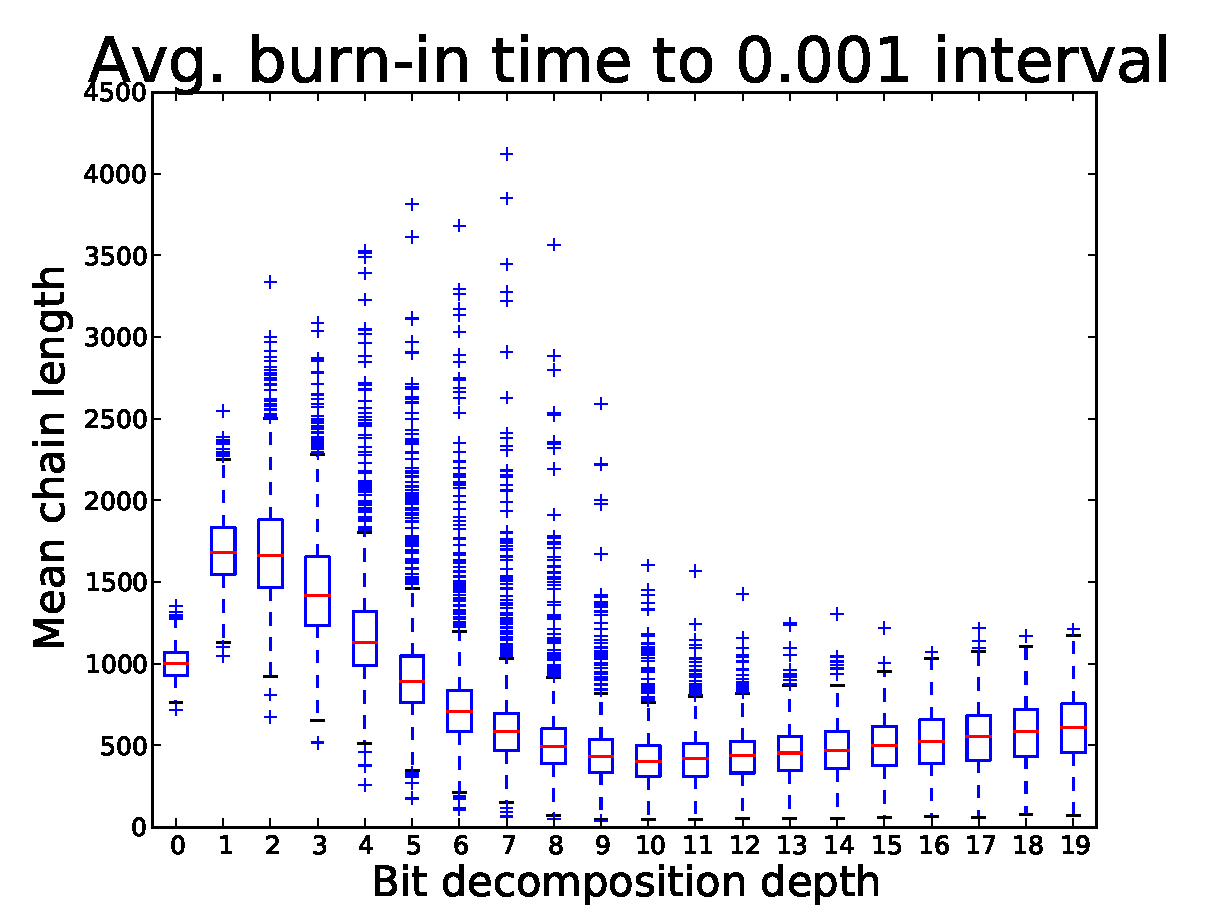
\includegraphics[width=\textwidth]{AllShiftsMax0001}
      \caption{Maximum sized shifts.}
      \label{fig:allMaxShifts}
    \end{subfigure}
    ~
    \begin{subfigure}[t]{0.48\textwidth}
      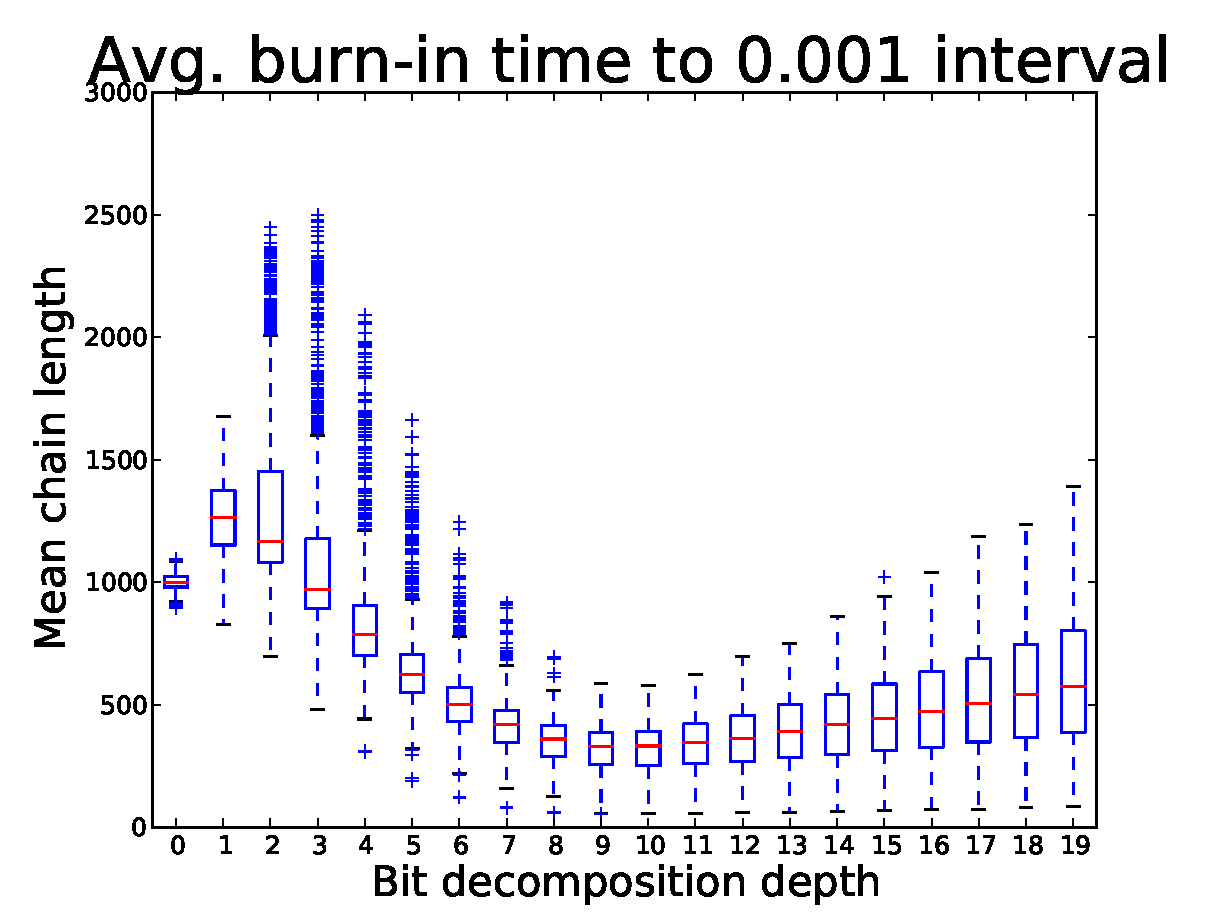
\includegraphics[width=\textwidth]{AllShiftsMin0001}
      \caption{Minimum sized shifts.}
      \label{fig:allMinShifts}
    \end{subfigure}
    \caption{Time to 0.001 neighbourhood of mode, averaged over all mode placements, for bit decompositions of different depths using a shift for every bit.}
    \label{fig:allShifts}
\end{figure}


As explained in Section \ref{sect:stuckMath}, the shift size $s$ for bit $k$ needs to respect $2^{-k-1} <= s <= 2^{-k}$ in order for us to be able to jump to the mode in one step. In \ref{fig:allMinShifts} we check whether the choice of shift size within this interval is significant, by looking at the burn-in rate for shifts of size $2^{-k-1}$ (called minimum shifts) for each bit position k. The results are quite similar to those obtained for the maximum shifts, which suggests that the performance isn't sensitive to the choice of shift length within $[2^{-k-1}, 2^{-k}]$.

We would also like to see what happens as the size of the target neighbourhood changes. In Figure \ref{fig:AllShiftsMax001} we repeat the max shift experiment for a target neighbourhood of size 0.01 (10x larger). While the bit decomposition still gives some advantage, as the size of the target neighbourhood increases this advantage appears to become less significant. Intuitively this happens because a larger number of the less significant bits become irrelevant as far as ending up in the desired region is concerned.

\begin{figure}[h]
    \centering
    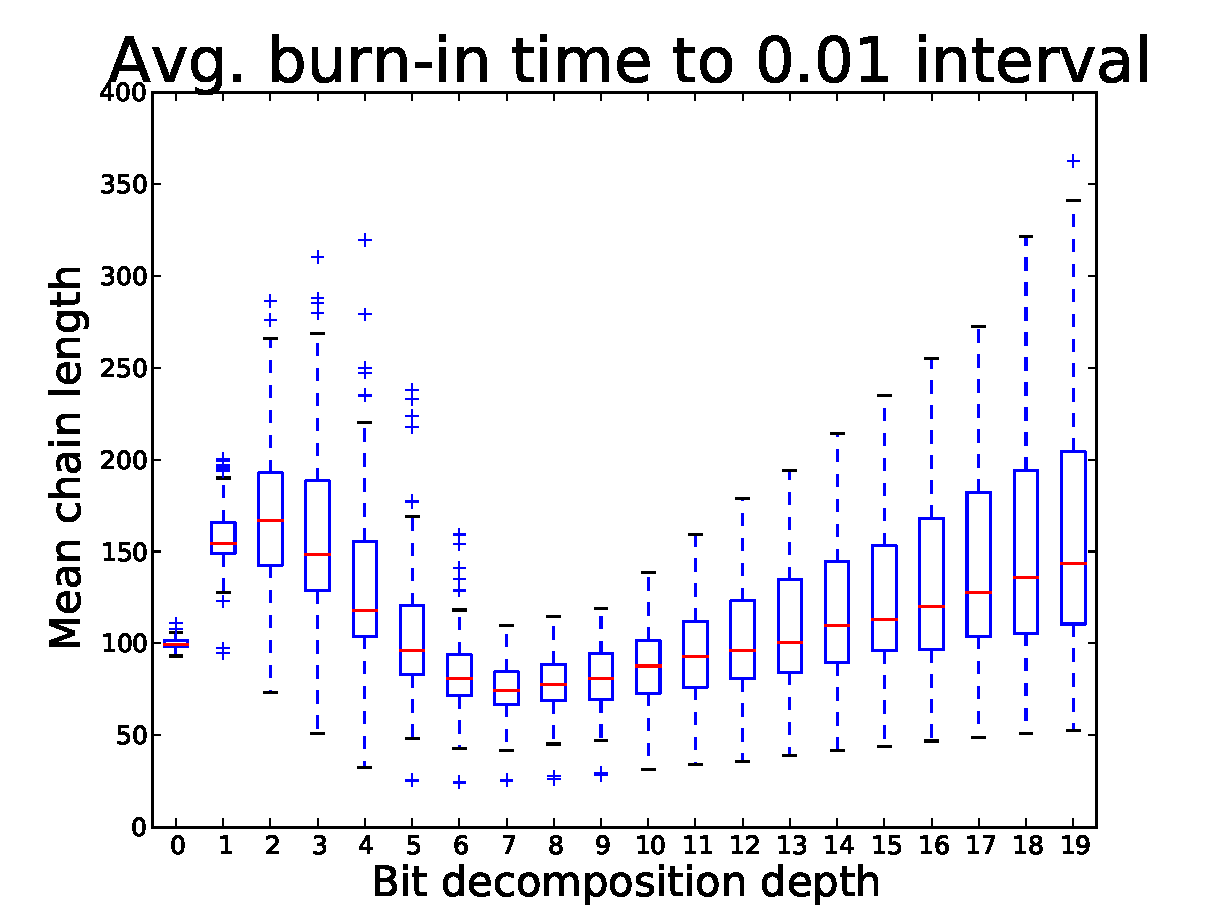
\includegraphics[width=0.8\textwidth]{AllShiftsMax001}
    \caption{Time to 0.01 neighbourhood of mode, averaged over all mode placements, for bit decompositions of different depths using a shift for every bit.}
    \label{fig:AllShiftsMax001}
\end{figure}

Finally, we would also like to see what happens to the performance if we do not provide k shifts for k bits, but instead only 1 or 2 shifts. As explained in section \ref{sect:stuckMath}, a single properly sized shift is sufficient to stop us from getting stuck. However, without k shifts for k bits, we sacrifice the ability of always moving from a stuck position to the mode in one step. As seen in Figure \ref{fig:fewShifts}, this seems to have a significant negative effect on the decompositions' performance. \todo{talk about distributions over shifts, and more about benefits/drawback of shifts and/or changing depths}

\begin{figure}[h]
    \centering
    \begin{subfigure}[t]{0.48\textwidth}
      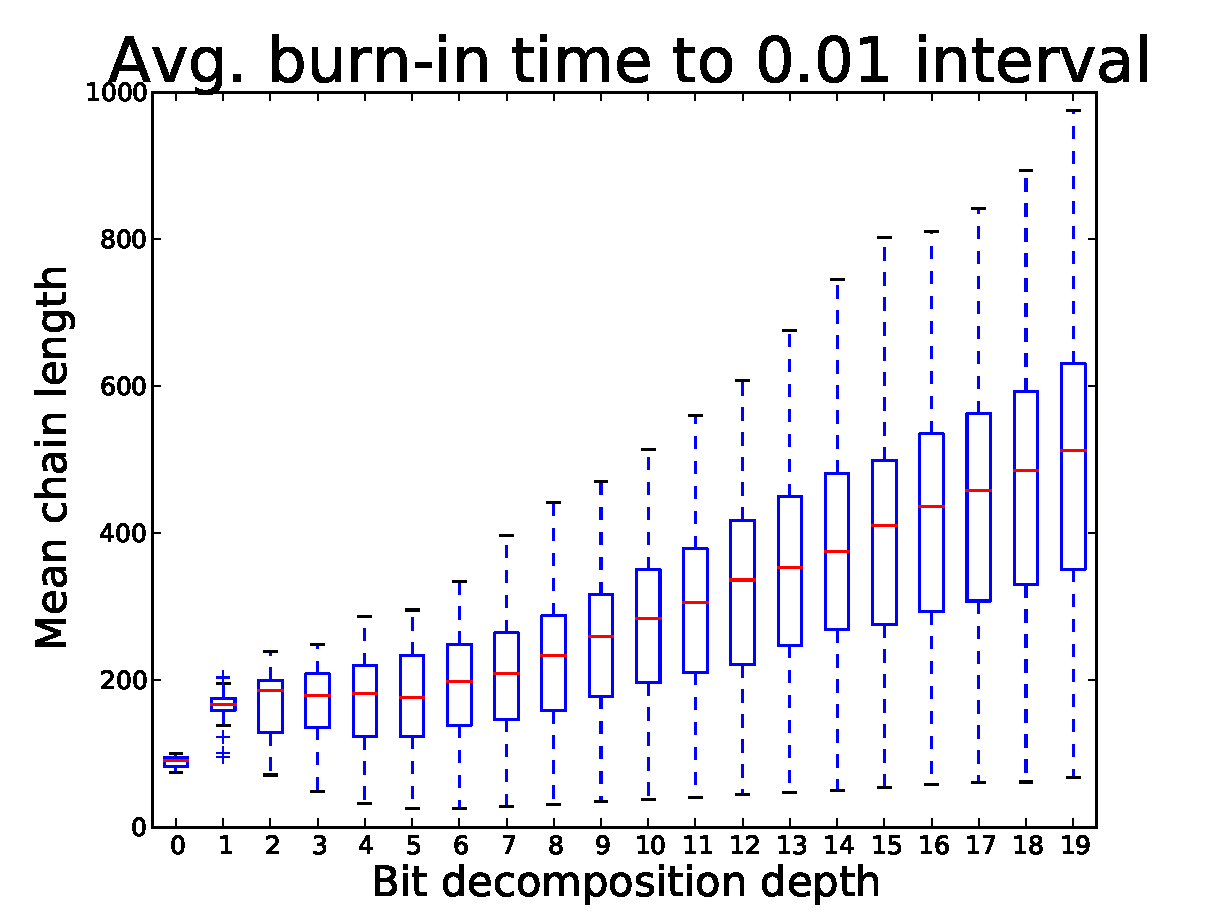
\includegraphics[width=\textwidth]{05Shift001}
      \caption{Shift of size 0.5}
    \end{subfigure}
    ~
    \begin{subfigure}[t]{0.48\textwidth}
      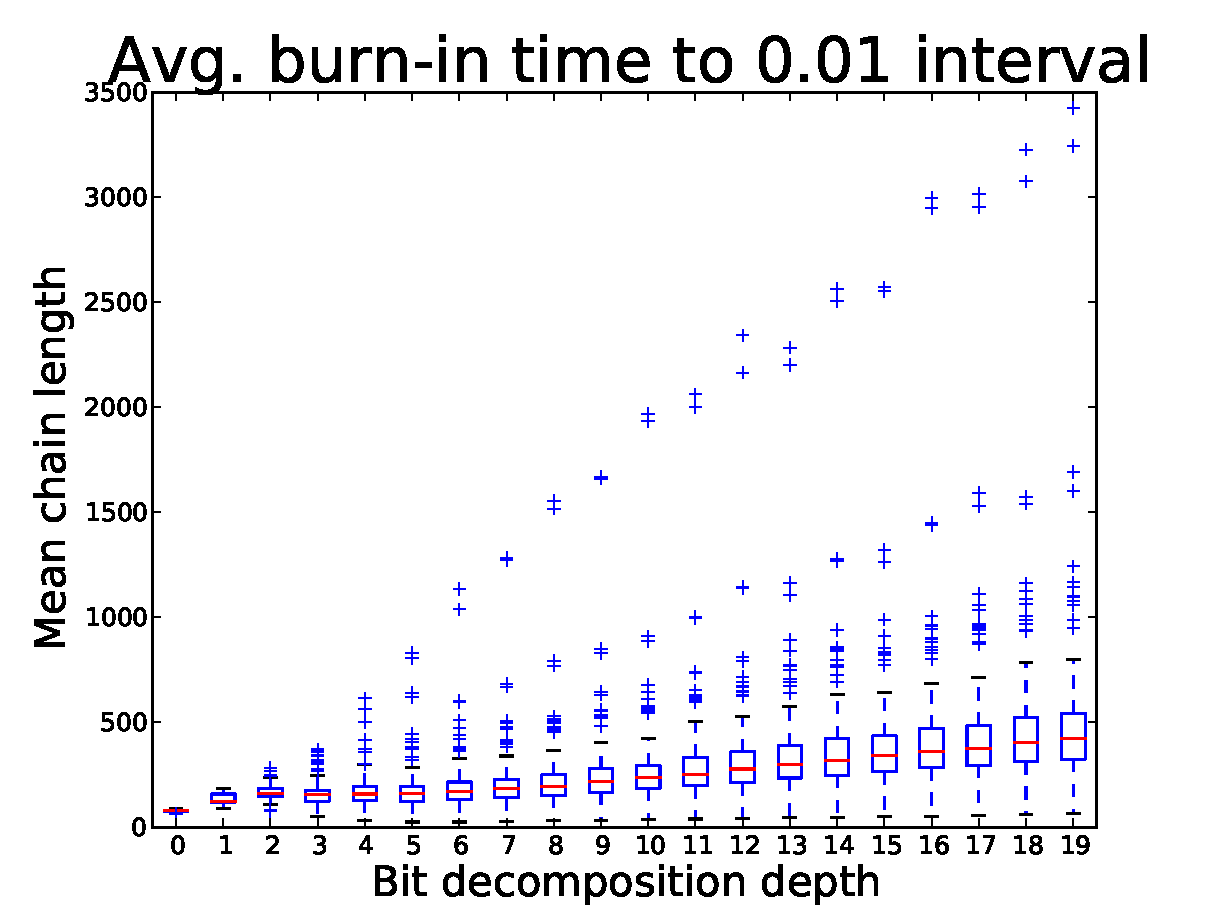
\includegraphics[width=\textwidth]{02505Shift001}
      \caption{Shift of size 0.25 and 0.5}
    \end{subfigure}
    \caption{Time to 0.01 neighbourhood of mode, averaged over all mode placements, for bit decompositions of different depth using a small number of shifts.}
    \label{fig:fewShifts}
\end{figure}

\subsubsection{Determining optimal shifts and shift transitions}
It seems we have a wide variety of options regarding what shifts to use and how to transition between them. It therefore seems worthwhile to consider the question of whether we can determine any optimal solutions analytically. 

In order to do so, we make some observations:
\begin{itemize}

\item
The location of the mode neighbourhood determines which regions are traps (i.e. in which regions, once you enter, you can no longer reach the mode without shifting)

\item
The current sample determines what portion of the traps (if any) are still accessible (based on the assumption that it is arbitrarily unlikely for the log-likelihood to decrease between consecutive samples).

\item
The probability of getting to the mode or falling in a trap cannot be modelled with (mixtures of) geometric distributions since a sample's probability distribution depends on the previous samples (and is therefore not uniform, unless we integrate out its history)

\item
For a set mode and log-likelihood function we can represent the transition between samples via a bit-level markov chain which ignores the trailing uniform. We can then create absorbing states representing the mode neighbourhood and the traps.

\item
If, for instance, the neighbourhood is only 0.1 of the length of the smallest bit we would implicitly represent the uniform only in the corresponding bit state by giving a 0.1 transition from this bit state to the mode-neighbourhood absorbing state. This however ignores the movement of the uniform during normal sampling which may end up biasing the results since, for instance, if the mode is in the leftmost bit the uniform will likely already have a very small value by the time the correct bit state is reached. \todo{There seem to be heuristic ways to address this}

\item
Using this formulation we can analytically derive the probability of getting stuck and the expected number of steps to the mode. Representing shifted priors is also possible. The simplest way would be to have 2x the nodes for a combination of 2 shifted priors.

\end{itemize}
\todo{try to get some results using markov chain implementation. Otherwise there's not much point in describing it ...}


